%%
%% This is file `sample-sigconf.tex',
%% generated with the docstrip utility.
%%
%% The original source files were:
%%
%% samples.dtx  (with options: `sigconf')
%% 
%% IMPORTANT NOTICE:
%% 
%% For the copyright see the source file.
%% 
%% Any modified versions of this file must be renamed
%% with new filenames distinct from sample-sigconf.tex.
%% 
%% For distribution of the original source see the terms
%% for copying and modification in the file samples.dtx.
%% 
%% This generated file may be distributed as long as the
%% original source files, as listed above, are part of the
%% same distribution. (The sources need not necessarily be
%% in the same archive or directory.)
%%
%% The first command in your LaTeX source must be the \documentclass command.
\documentclass[sigconf, table]{acmart}

%%
%% \BibTeX command to typeset BibTeX logo in the docs
\AtBeginDocument{%
  \providecommand\BibTeX{{%
    \normalfont B\kern-0.5em{\scshape i\kern-0.25em b}\kern-0.8em\TeX}}}



%%%%%%%%%%%%
\copyrightyear{2020}
\acmYear{2020}
\setcopyright{acmcopyright}
\acmConference[e-Energy'20]{The Eleventh ACM International Conference on Future Energy Systems}{June 22--26, 2020}{Virtual Event, Australia}
\acmBooktitle{The Eleventh ACM International Conference on Future Energy Systems (e-Energy'20), June 22--26, 2020, Virtual Event, Australia}
\acmPrice{15.00}
\acmDOI{10.1145/3396851.3397729}
\acmISBN{978-1-4503-8009-6/20/06}
%%%%%%%%%%5

\usepackage{optidef}
%\usepackage[table]{xcolor}

\usepackage{tikz}
\usepackage{pgfplots}
\usetikzlibrary{math}
\usetikzlibrary{calc}
\usetikzlibrary{decorations.pathreplacing, matrix}
\usetikzlibrary{pgfplots.statistics}
\pgfplotsset{compat=1.16}

\newcommand{\N}{\mathcal{N}}
\newcommand{\Bat}{\mathcal{B}}
\newcommand{\Ep}{E^+}
\newcommand{\Ene}{E^-}
\newcommand{\ep}{e^+}
\newcommand{\ene}{e^-}
\newcommand{\pricelow}{p^l}
\newcommand{\pricehigh}{p^h}
\newcommand{\costbat}{\pi}
\newcommand{\bat}{B}
\newcommand{\ramp}{\delta}
\newcommand{\cons}{x}
\newcommand{\coef}{\gamma}

\newcommand{\floor}[1]{\left\lfloor #1 \right\rfloor}
\newcommand{\ceil}[1]{\left\lceil #1 \right\rceil}


\newcommand{\ccd}{c_{cd}}
\newcommand{\acd}{A_{cd}}
\newcommand{\bcd}{b_{cd}}
\newcommand{\ccs}{c_{cs}}
\newcommand{\acs}{A_{cs}}
\newcommand{\bcs}{b_{cs}}
%%
%% Submission ID.
%% Use this when submitting an article to a sponsored event. You'll
%% receive a unique submission ID from the organizers
%% of the event, and this ID should be used as the parameter to this command.
%%\acmSubmissionID{123-A56-BU3}

%%
%% The majority of ACM publications use numbered citations and
%% references.  The command \citestyle{authoryear} switches to the
%% "author year" style.
%%
%% If you are preparing content for an event
%% sponsored by ACM SIGGRAPH, you must use the "author year" style of
%% citations and references.
%% Uncommenting
%% the next command will enable that style.
%%\citestyle{acmauthoryear}

%%
%% end of the preamble, start of the body of the document source.


\pgfplotscreateplotcyclelist{mycycle}{
black, fill=red!40,every mark/.append style={fill=blue!80!black},mark=*\\
}

\begin{document}

%%
%% The "title" command has an optional parameter,
%% allowing the author to define a "short title" to be used in page headers.
\title{Discrete and stochastic coalitional storage games}

%%
%% The "author" command and its associated commands are used to define
%% the authors and their affiliations.
%% Of note is the shared affiliation of the first two authors, and the
%% "authornote" and "authornotemark" commands
%% used to denote shared contribution to the research.
\author{Diego Kiedanski}
\email{diego.kiedanski@telecom-paristech.fr}
\orcid{1234-5678-9012}
\affiliation{%
  \institution{T\'el\'ecom Paris}
  \streetaddress{}
  \city{Palisseau}
  \state{France}
}

\author{Ariel Orda}
\email{ariel@ee.technion.ac.il} 
\affiliation{%
  \institution{Technion}
  \city{Haifa}
  \country{Israel}}


\author{Daniel Kofman}
\email{daniel.kofman@telecom-paristech.fr}
\affiliation{%
  \institution{T\'el\'ecom Paris}
  \streetaddress{}
  \city{Palisseau}
  \state{France}
}
%%
%% By default, the full list of authors will be used in the page
%% headers. Often, this list is too long, and will overlap
%% other information printed in the page headers. This command allows
%% the author to define a more concise list
%% of authors' names for this purpose.
\renewcommand{\shortauthors}{D. Kiedanski, A. Orda, D. Kofman.}

%%
%% The abstract is a short summary of the work to be presented in the
%% article.
\begin{abstract}
%To achieve a fully decarbonized power grid, a massive deployment of renewable energy resources will be needed, but because of the intermittent nature of their generation, their full potential will not be unleashed unless demand side flexibility plays a bigger role than today.

%Introducing energy storage at the residential level enables increasing load flexibility, as it allows end-customers to easily change their consumption profile and adapt to the grid requirements.

As of today, energy storage for residential consumers represents a considerable investment that is not guaranteed to be profitable. Shared investment models in which a group of consumers jointly acquires energy storage have been proposed in the literature to increase the attractiveness of these devices. Such models naturally employ concepts of cooperative game theory.

In this paper, we extend the state-of-the-art cooperative game for modeling the shared investment in storage by adding two crucial extensions: {\em stochasticity} of the load and {\em discreetness} of the storage device capacity.
As our goal is to increase storage capacity in the grid, the number of devices that would be acquired by a group of players that cooperate according to our proposed scheme is compared to the number of devices that would be bought by consumers acting individually. 
Under the same criteria of customer profitability,
simulations using real data reveal that our proposed scheme can increase the deployed storage capacity between $100\%$ and $250\%$.
\end{abstract}

%%
%% The code below is generated by the tool at http://dl.acm.org/ccs.cfm.
%% Please copy and paste the code instead of the example below.
%%

\begin{CCSXML}
<ccs2012>
<concept>
<concept_id>10003752.10010070.10010099.10010102</concept_id>
<concept_desc>Theory of computation~Solution concepts in game theory</concept_desc>
<concept_significance>500</concept_significance>
</concept>
<concept>
<concept_id>10010583.10010662.10010663.10010664</concept_id>
<concept_desc>Hardware~Batteries</concept_desc>
<concept_significance>500</concept_significance>
</concept>
</ccs2012>
\end{CCSXML}

\ccsdesc[500]{Theory of computation~Solution concepts in game theory}
\ccsdesc[500]{Hardware~Batteries}


%%
%% Keywords. The author(s) should pick words that accurately describe
%% the work being presented. Separate the keywords with commas.
\keywords{Smart Grids, Energy Storage, Battery, Prosumer, Cooperative Game Theory, Shared Investment, Sharing Economy}

%% A "teaser" image appears between the author and affiliation
%% information and the body of the document, and typically spans the
%% page.


%%
%% This command processes the author and affiliation and title
%% information and builds the first part of the formatted document.
\maketitle

\begin{acks}
The VALADOE Chair of IMT Atlantique in partnership with Télécom ParisTech and Mines Saint Etienne and supported by ENEDIS, Région Pays de la Loire, Nantes Metropole
This publication only reflects the views of its author(s). Neither the ValaDoE Steering Committee nor the associated organizations can be held responsible for the use that could be made of the information contained therein.
\end{acks}



\section{Introduction}

The imminent threat of climate change requires the replacement of CO2 producing energy resources by renewables such as solar and wind. Unfortunately, the intermittent nature of such sources limits their massive adoption.
As energy production and consumption need to be balanced at all times, one of the solutions to mitigate this issue is to deploy energy storage in the power grid.
At the residential level, the rate of storage adoption is slower than desired. Although many battery products exist, the corresponding investment is today rarely profitable.
An end-customer can benefit from having storage by coupling it with local renewable energy production or even without that, if the electricity tariff is designed in such a way that the storage enables a smart shift in the overall consumption pattern. 
Even if a consumer can reduce her/his electricity cost by charging the battery during the cheap electricity hours and discharging it during the most expensive ones, it might not be enough to offset the initial cost of the battery.
If the battery is underused, the end-consumer might be able to team with neighbours and jointly invest in the storage, thus reducing the burden of the initial investment.
This idea, of shared investment in storage, has already been proposed, and preliminary studies indicate that it may be highly beneficial.
One major problem associated with such an investment is how to share the costs among customers.
Indeed, if there is a big difference among the energy usage patterns of the involved consumers, some of the participants will be unwilling to contribute equally to the cost.
Therefore, a central question to the idea of a shared investment in storage is whether there exists a \textit{stable} way to divide the total costs, such that no participant has an incentive to opt out of the investment agreement.

A natural tool to study such problems is cooperative game theory. In a cooperative game, a set of players considers the benefits of forming a coalition with every other group of players. A solution to the game is a distribution of the total benefits among all players such that no subset of players wishes to deviate, i.e., abandon the other members of the group and invest on their own.
In this study, we extend previous formulations of such shared investment models so as to bridge the theory with its applicability. Specifically, while previous studies focused on deterministic energy consumption profiles, we consider the broader (and more realistic) framework of stochastic profiles; furthermore, while previous studies assumed that any fraction of a battery can be bought, we introduce realistic constraints regarding the discrete sizes of batteries.
We then prove that, for the stochastic yet continuous case, a solution of the game always exists and we provide an efficient algorithm to find it. On the other hand, we show that the discrete case may fail to admit a solution. Accordingly, for that case, we provide an approximate solution that appears to be satisfactory for real-world deployments. 
Our algorithm is based on the solution of a linear optimization problem hence it is able to scale to large numbers of players.
%Until know, the core as a solution was sometimes avoided because of the computational complexity of finding it. In this regards, our method provides, as far as we know, the first computationally efficient study of the core for coalitional games.

The rest of the paper is organized as follows. Section 2 positions our work within the literature. Section 3 describes coalitional games at the detail required to present the remaining sections.
Section 4 establishes the existence of a solution for the continuous, deterministic case. The result is then extended in Section 5 for the stochastic, yet still continuous, case.
We consider the inherent discreteness of the battery size and its implications on our model in Section 6. Numerical simulations are presented in Section 7. Finally, Section 8 presents concluding remarks.
% With the rapid development of renewable energy resources, it beomes increasingly complicated to operate the grid and to balance consumption and generation. The need for storage is more obvious than ever but it is still not clear whether some of those investments are profitable.
% Several new technologies targeting different needs have appared, but until the new technologies get fully deployed, we might have to wait extra 10 yeras.

% When trying to find solutions that result in a deployment of solar today, the idea of share storage has been explored. Such solutions have proven to be very useful.


% In this paper we develop on the mathametical tools available for this problem and provide several extension and bridge the theory and the future application of such models

\section{Related Work}

It appears that the first proposal to use cooperative game theory to model the shared investment in storage is \cite{chakraborty2018}, which introduced the idea of coalitional storage games. That study did not consider ramp constraints; that is, it was assumed that the battery could be fully charged or discharged instantly. That study did model the load as stochastic, yet because of the absence of ramp constraints, it was sufficient to only consider the total consumption in a day and not the intra-day consumption of each player. It was then proven that the considered game admits a non-empty core, and a closed-form solution that belongs to the core was provided.

In \cite{kiedanskigames}, the formulation of \cite{chakraborty2018} was extended to include ramp constraints. That study identified families of games with non-empty cores as well as families of convex games. Nevertheless, \cite{kiedanskigames} did not ensure the existence of non-empty cores for all games, nor it considered stochastic load profiles or discrete battery sizes.

%For the new formulation, and some families of games they proved the existence of solutions such as the core  and studied different families of such games, but did not prove the existence in the general case, nor they dealt with stochastic consumption or discrete battery sizes.

The present work extends upon the above line of studies, by considering stochastic load profiles and discrete battery sizes, for which we prove that a stable (or almost-stable) solution exists, i.e., the core is not empty.

The study \cite{RePEc:cam:camdae:1740} looked at the joint investment in photo-voltaic panels by a group of neighbours. It was shown that, under certain assumptions on the consumption profiles, the resulting game is convex. An extension of \cite{RePEc:cam:camdae:1740} was presented in \cite{RePEc:cam:camdae:1828:snowball}, which included investment in batteries too. The results of \cite{RePEc:cam:camdae:1740} do not hold when also taking into account storage, hence, \cite{RePEc:cam:camdae:1828:snowball} mostly focused on the relationship between the formation of communities and the electricity tariff, and on how changes in one can trigger changes in the other.

The study \cite{hedonic} also considered cooperative games for energy sharing. But instead of looking at the investment problem, it was assumed that players already own the equipment and are interested in sharing it. 
Specifically,  \cite{hedonic} considered Hedonic games, a class of cooperative games without transferable utilities, i.e., there is no money exchanged between players. One interesting aspect of \cite{hedonic} is that it considered two scenarios: sharing energy by creating a specific grid and by using the existing grid. In our work, we deal with the latter type of settlements.

The ideas presented in the present work are also related to the literature on optimal battery sizing. In \cite{KHALILPOUR2016194}, a mixed integer linear optimization problem is formulated to decide on the optimal size of a storage/photo-voltaic system. A similar but stochastic formulation was presented in \cite{CERVANTES2018105}. 
Our optimization problem is formulated in a similar way, with the inherent difference that it is embedded in a cooperative game.
%Their optimization problem resembles the one used in Section \ref{sec:stoc} of this paper.
%This model requries data and for such cases...
Approaches to optimal battery sizing require a considerable amount of consumption data. If such information is not available, synthetic data can be generated and used instead, as proposed in \cite{synthetictraces}.
%More complex tasks, such as generating synthetic data to improve the investment decision are studied in , but they are out of the scope of our paper.
%In general, using ideas of the sharing economy \cite{sharingeconomy}, already popularized by companies such as Airbnb \cite{oskam2016airbnb} in the Smart Grid has been increasing in popularity.

\section{Preliminaries}

\subsection{Cooperative Game theory}

A cooperative game $G$ can be defined as a tuple $G = (\N, v)$, where $\N = \{1, \dots, N\}$ is the set of players and $v \colon 2^N \to \mathbb{R}$, specifies for each coalition S (subset of the $\N$ players) what the total cost incurred by them is.
In general, we assume that $v(\emptyset) = 0$ and furthermore we refer to the set of all players as the Grand Coalition $S = \N$.

The solution of a cooperative game $G$ is a payoff vector $y \in \mathbb{R}^N$ that specifies how much each player should pay. The coordinate $j$ of $y$, $y_j \in \mathbb{R}$, specifies how much player $j$ should pay while taking part in the Grand Coalition. We seek payoffs that satisfy good properties and guarantee some kind of stability.

\begin{definition}\label{def:pg_ir}
  A payoff vector $y$ is {\em individually rational} if $y_i \leq v(\{i\})$, i.e, the player is better off by participating in the grand coalition.
\end{definition}

\begin{definition}\label{def:pf_gr}
  A payoff vector $y$ is {\em group rational} if $\sum_{j \in S} y_j \leq v(S)$. That is, all players pay less than if they formed the coalition $S$. Observe that if this was not the case, they would have an incentive to leave the grand coalition and receive $v(\{S\})$.
\end{definition}

\begin{definition}\label{def:pf_eff}
 A payoff vector $y$ is {\em efficient} if $\sum_{i \in S} y_i = v(N)$.
\end{definition}

\begin{definition}\label{def:imputation}
  A payoff vector that is both efficient and individually rational is called {\em an imputation}.
\end{definition}

\begin{definition}\label{def:core}
  The {\em core of a game} is the set of imputations that are group rational.
\end{definition}

The core is a central solution concept in cooperative game theory. Indeed, knowing that a payoff is in the core guarantees a certain sense of stability.
The core can be empty, in which case no \textit{stable} solution exists. Deciding whether the core is empty is in general an NP-complete problem \cite{deng1994complexity}.

A general tool to check if the core is empty or not is due to Bondareva and is presented in Theorem \ref{th:bondareva}.

\begin{theorem}\label{th:bondareva}
 (Bondareva) A cooperative game $G = (\N, v)$ has a nonempty core if and only if every function $\alpha \colon 2^N \setminus \{\emptyset\} \to [0, 1]$ that satisfies Equation \eqref{eq:balanced} also satisfies the condition stated in Equation \eqref{eq:balanced_core} \cite{bondareva}.

\begin{equation}
\label{eq:balanced}
\forall i \in \N \colon \sum_{S|i \in S} \alpha(S) = 1
\end{equation}
\end{theorem}

\begin{equation}
\label{eq:balanced_core}
\sum_{S \in 2^{\N} \setminus \{\emptyset\}} \alpha(S)v(S) \geq v(N)
\end{equation}

A more detailed introduction to cooperative game theory can be found in \cite{rapoport1970n}.

\subsection{Coalitional Storage Games}

In this subsection we introduce the coalitional storage game defined in \cite{kiedanskigames}, which we shall use as the base model for the extensions developed in this study.

Consider a coalition of players $S \subset \N$, where $\N$ is the set of all players.
The aggregated energy consumption of $S$ is denoted by $x^S$. Because we only observe the consumption at discrete time intervals, we will denote by  $x^S_t$ the net consumption of $S$ at time-slot $t = 1, \dots, \mathcal{T}$, where $\mathcal{T}$ is the maximum number of time-slots in a single day (for $15$ minutes time intervals, $\mathcal{T}=96$).
All players are subject to an electricity tariff $p$, where $p_t$ denotes the price of $1 kWh$ at time-slot $t$.
%It is assumed that all players face the same electricity tariff $p$ offered by some utility company and that $p^l = p_{t_1} < p_{t_2} = p^h$ for some $1 \leq t_1 < t_2 \leq \mathcal{T}$. Without loss of generality, we will assume that the change in prices occurs at $\mathcal{T}\frac 1 2$.

Under the above scenario, the cost of a coalition $S$ without a battery is given by Equation \eqref{eq:cost_coal_nobat}. That is, the cost is given exactly by their electricity price, i.e.:

\begin{equation}
  \label{eq:cost_coal_nobat}
  c^S(0) \overset{\Delta}{=} \sum_{t=1}^{\mathcal{T}} p_t x^S_t
%  c^S(0) = p^l\sum_{t=1}^{\frac{\mathcal{T}}{2}} x^S_t + p^h\sum_{\frac{\mathcal{T}}{2}}^{\mathcal{T}}x^S_t
\end{equation}

Next, we introduce batteries and their potential application. Let $\Bat = (B, P, L, \delta)$ be a battery with capacity $B$ that costs $P$ per $kWh$, lasts $L$ days and has a maximum charge rate of $\delta$ (again, to simplify notation, we assume that the discharging capacity is $-\delta$).

A coalition $S$ can benefit from owning a battery if there exists $p_i < p_j$ with $i < j$, such that the coalition can charge at time-slot $i$ the energy consumption of time-slot $j$: $x^S_j$.

Following the conventions in \cite{kiedanskigames}, we will assume that the cost of buying a battery is linear in the capacity. Furthermore, the electricity tariff takes two values: $p_t = \pricelow, \ t=1, \dots, \frac{\mathcal{T}}{2}$ and $p_t = \pricehigh, \ t=\frac{\mathcal{T}}{2} + 1, \dots, \mathcal{T}$ with $\pricelow < \pricehigh$.
Accordingly, the cost of a coalition within a single day and with the battery $\Bat$ is now given as follows:

\begin{equation}
  \begin{aligned}
  \label{eq:cost_coal_bat}
  v^S(\Bat) &\overset{\Delta}{=} \frac{BP}{L} + p^l\sum_{t=1}^{\frac{\mathcal{T}}{2}} x^S_t
  + p^ h\sum_{t=\frac{\mathcal{T}}{2} + 1}^{\mathcal{{T}}} x^S_t \\
  &- (p^h -p^l)\min\left\{ B, \sum_{t=\frac{\mathcal{T}}{2} + 1}^{\mathcal{{T}}} \min\{x^S_t, \delta B\} \right\} \\
  \end{aligned}
\end{equation}

%If it is clear which battery product the game is played with, we shall also use the notation $v^S$ or $v(S)$ to denote $v^S(\Bat)$.

Finally, the cost of a coalition $S$ corresponds to an optimal investment in a battery, namely:

\begin{equation}
  \label{eq:cost_coal}
  v(S) = v^S \overset{\Delta}{=} \min_{B'} v^S(\Bat(B'))
\end{equation}

where the minimization is done using the battery size as the only parameter that changes. In the continuous version of the problem, any non-negative value of $B$ is valid. However, in the discrete version, only multiples of the original battery size are allowed: $B' = kB, k \in \mathbb{N}$. We will often refer to the coaltional game that allows any real positive value for the battery capacity as the \textit{continous version} of the game and to the games where we only allow for multiples of the original battery size as \textit{discrete} games.

Given the above (base) model of \cite{kiedanskigames}, we shall present a new and more convenient formulation of the same game that will enable us to prove the main theoretical results of this study.
%turn to present the extended model that is the subject of the present work.


%\section{Model Re-Formulation}

\section{Formulating Coalitional Storage Games as Linear Programs}

In the previous section, we defined the cost of a coalition in a coalitional storage game using the minimization problem present in Equation \eqref{eq:cost_coal}. Even though it is compact, the nested minimum structure in it does not make it amenable to the theoretical analysis that we wish to pursue in this paper. Therefore, we seek to find an equivalent but more useful way to represent the cost of each coalition.

In cooperative game theory, one of the most well known studied games are linear production games (LPG) \cite{Borm2001}, \cite{Owen1975}. In this class of games, each player has some resources and the value of each coalition is determined by how much the coalition can produce with the collection of the resources of all its players.
In LPG, the cost of each coalition is given by a linear program and by exploiting the duality of such linear programs it can be proven that all LPGs have non-empty cores. 
Inspired by these findings, we shall formulate the minimization problem in \eqref{eq:cost_coal} as a linear program and frame it as an LPG.



%As mentioned, we provide two major extensions to the model introduced in the previous section, namely: stochastic load profiles and discrete battery size. Both extensions rely on a reformulation of the minimization problem (Equation \eqref{eq:cost_coal}), which yields the cost of a coalition  as a linear program.

%As a first step, in this section we introduce the new formulation yet still without any extensions, i.e., the capacity of the battery bought may still be any positive number and the load is still deterministic. We use it to prove that the core of such games (as defined in \cite{kiedanskigames}) is non-empty: this is already a new result. We also show how to efficiently find a vector in the core.

%We shall show how the cost of a coalition in a coalitional storage game (Equation \eqref{eq:cost_coal}) admits a linear programming formulation. This shall enable us to show that, for the continuous version of the problem, the core is always not empty.

The linear programming problem equivalent to Equation \eqref{eq:cost_coal} that computes the cost of a coalition is given by Equation \eqref{eq:cost_lp}. The formulation does not include the cost that is normally incurred during the cheap period. This value is always constant and additive, hence to simplify the notation, from now onward we will assume that it is always $0$, i.e., $x^S_t = 0, t = 1, \dots, \frac{\mathcal{T}}{2}$.

\begin{mini!}[3]
{\bat, \Ep, \Ene, \ep, \ene}{\left[ \frac{P}{L} \bat + \pricelow(\bat - \Ene) +  \pricehigh(\Ep + \sum_t \ep_t)\right]}{}{Problem \ P^S)}\label{eq:cost_lp}
\addConstraint{\ramp\bat + \ep_t - \ene_t}{ = \sum_{n \in S} \cons^n_t}{ \ \forall t \in \mathcal{T}}{\quad (\lambda_t)}{\label{cons:ramp}}
\addConstraint{\bat + \Ep - \Ene}{= \sum_t (\ramp\bat - \ene_t)}{}{\quad (\mu)}
\addConstraint{\bat, \Ep, \Ene, \ep, \ene}{\geq 0}{}
\end{mini!}

The newly introduced variables are interpreted as follows:

\begin{enumerate}
    \item $\ep$: For each time slot, is the amount of energy required beyond the maximum ramp constraint.
    \item $\ene$: For each time slot is the amount of energy below the maximum ramp constraint.
    \item $\Ep$: Is the total amount of energy consumed beyond the battery capacity, taking into account only the energy that could be stored, i.e, ignoring the energy that requires more power than the ramp constraint.
    \item $\Ene$: Gap between the energy required and the total amount of energy in the battery.
    \item $\lambda_t$ and $\mu$ are the dual variables associated with each of the equations.
\end{enumerate}

\begin{proposition}\label{prop:equiv}
The optimization problems \eqref{eq:cost_coal} and \eqref{eq:cost_lp} are equivalent.
\end{proposition}

\begin{proof}

The proof can be found in Appendix \ref{ap:equiv}.

% The basic idea is as follows: each variable $\ep_t, \ene_t$ allows us to represent the minimum inside the summation in Equation \eqref{eq:cost_coal_bat}, while $\Ep, \Ene$ represent the outer minimum.

% Specifically, by Equation \eqref{cons:ramp}: $\min\{ \delta B, x^S_t \} = \min\{ \delta B, \delta B + \ep_t - \ene_t \} = \min\{ \delta B, \delta B - \ene_t \} = \delta B - \ene_t$. \\
% Doing some extra arithmetic we obtain that:

% \begin{equation*}
% \begin{aligned}
% &\min\left\{ B, \sum_{t=\frac{\mathcal{T}}{2}}^{\mathcal{{T}}} \min\{x^S_t, \delta B\} \right\} = \min\{ B, \sum_t \delta  B - \ene_t \}\\
% &= \min\{ B, B + \Ep - \Ene\} = B - \Ene
% \end{aligned}
% \end{equation*}

% \begin{equation}
%     \begin{aligned}
%       v^S(\Bat) &= \frac{BP}{L}   + p^ h\sum_{t=\frac{\mathcal{T}}{2}}^{\mathcal{{T}}} x^S_t 
%   - (p^h -p^l)(B - \Ene)   \\
%   &= \frac{BP}{L} + \pricelow (B - \Ene)   + p^ h\sum_{t \in \mathcal{T}} x^S_t - \pricehigh(B - \Ene) \\
%   & = \frac{BP}{L} + \pricelow (B - \Ene) + \pricehigh \sum_t (\delta B + \ep_t - \ene_t) \\
%   &- \pricehigh((\sum_t (\delta B - \ene_t) - \Ene) \\
%   & =  \frac{BP}{L} + \pricelow (B - \Ene) + \pricehigh (\Ep + \sum_t \ep)
%     \end{aligned}
% \end{equation}

\end{proof}



\begin{proposition}
The optimization problem \eqref{eq:cost_lp} can be written as: $\min\{ \ccd x \colon \acd x = \bcd , x \geq 0\}$, where the superscript $cd$ denotes that it is the matrix notation of the continuous and deterministic version of the problem. The explicit formulation is in Appendix \ref{ap:matrix}.
\end{proposition}

Even though the game of interest did not turn out to be exactly a Linear Production Game, we can still harness the main techniques used in LPG and apply them to our problem. We present the first result in that respect in Theorem \ref{th:core-cd}.

\begin{theorem}\label{th:core-cd}
  The cooperative game in which the cost of each coalition is given as the solution of the optimization problem \eqref{eq:cost_lp} satisfies the hypothesis of \ref{th:bondareva} and therefore it has a non-empty core.
\end{theorem}

\begin{proof}
We will show that the game is balanced. Then, through a direct application of the Bondareva-Shapley theorem \cite{Shapley1971}, it follows that the core is not empty.


Let $\alpha$ satisfy condition \eqref{eq:balanced}.

We begin by showing that $ \sum_S \alpha(S) x^S_t = x^N_t$. This fact follows simply by the application of the definition of $\alpha$ and it is proven as follows:
 

\begin{equation}\label{eq:rhs_core_deter}
    \begin{aligned}
        \sum_S \alpha(S) x^S_t & = \sum_S \alpha(S) \sum_{n \in S}x^n_t \\ &= \sum_{n \in N}x^n_t\sum_{S \colon i \in S} \alpha(S) \\ &= \sum_{n \in N} x^n_t = x^N_t
    \end{aligned}
 \end{equation}

Let $y_S$ denote an optimal solution of \eqref{eq:cost_lp} when solving for coalition $S$. Then:

\begin{equation}
    \sum_{S} \alpha(S) v(S) = \sum_{S} \alpha(S) \left(\ccd y_S\right) = \ccd \left(\sum_S \alpha(S) y_S \right)
\end{equation}

Now,

\begin{equation}
  \begin{aligned}
&    \acd \left(\sum_S \alpha(S) y_S \right) = \sum_S \alpha(S) \left( \acd y_S \right) = \\ &= \sum_S \alpha(S) \begin{bmatrix} x^S_1 \\ x^S_2 \\ \vdots \\ x^S_T \\ 0 \end{bmatrix} = \begin{bmatrix} \sum_S \alpha(S) x^S_1 \\ \sum_S \alpha(S) x^S_2 \\ \vdots \\ \sum_S \alpha(S) x^S_T \\ \sum_S \alpha(S) 0 \end{bmatrix} = \begin{bmatrix} x^N_1 \\ x^N_2 \\ \vdots \\ x^N_T \\ 0 \end{bmatrix}
    \end{aligned}
\end{equation}

Consequently, $\sum_S \alpha(S) y_s$ is a feasible solution of $P_N)$ (the optimization problem \eqref{eq:cost_lp} associated with the Grand Coalition). Moreover, because $v(N)$ is the minimum of that problem, it holds that 
\[
  \ccd \left(\sum_S \alpha(S) y_S \right) \geq v(N)
 \].
 
 This completes the proof.

\end{proof}

Although the core of a game is probably the most well-studied equilibrium concept in cooperative game theory, its main limitation is that, in general, it is $NP-complete$ to find an imputation in the core. This is a consequence of the fact that the number of constraints that define the core grows exponentially with the number of players.

Fortunately, borrowing ideas from the literature on linear production games, we can obtain an element of the core by solving a simple optimization problem. The idea is captured in the following theorem.

\begin{theorem}\label{th:payoff_cd}

  The payoff vector defined as $y = (u_1, u_2, \dots, u_N)$ where $u_i$ is defined as in Equation \eqref{eq:payment_dual_i} is in the core when the cost of each coalition is given by the optimization problem \eqref{eq:cost_lp}.

\end{theorem}

\begin{proof}

Consider the dual of the Linear Program defined in \eqref{eq:cost_lp}. Observe that the only dependence on the coalition $S$ is given by the vector $\bcd$, while $\acd$ as well as $\ccd$ do not depend on $S$. This has an important consequence: the solution of the optimization problem \eqref{opt:dual_cd}, defined for coalition $S$, is feasible for any other subset $U \subset \N$.

\begin{maxi!}[4]
{w}{\bcd(S)^Tw}{}{Problem \ D_S)}\label{opt:dual_cd}
\addConstraint{\acd^T w}{\leq \ccd}{}
\end{maxi!}

Let $w^*(N)=(w_1^*(N), \dots, w_{T+1}^*(N)$ be the optimal solution of the dual of the grand coalition. Due to duality, the following equalities hold:

\begin{equation}\label{eq:dual_sum_core}
 \begin{aligned} 
&\sum_{j=1}^{T} w_j^*(N)x^N_{j} + w_{T+1}^*(N)0 = v(N) \\
&\sum_{j=1}^{T} w_j^*(N)\sum_{i \in N}x^i_j = v(N) \\
 \end{aligned}
\end{equation}

%Remembering that for any vector in the core, the sum of the payoffs of all players has to be equal to $v(N)$ and using the last equality in Equation \eqref{eq:dual_sum_core}, we proceed to propose $u_i$ as defined in Equation \eqref{eq:payment_dual_i} as the cost of user $i$.
%We employ the above in order to define a payoff vector $y$ such that the cost paid by user $i$ as in Equation \eqref{eq:payment_dual_i}. The payment of user $i$ is proportional to his consumption in every times-slot.
%One can use the last equality in Equation \eqref{eq:dual_sum_core} 
We proceed to define a vector $y = (u_1, \dots, u_N)$ where each coordinate $u_i$ is given by Equation \eqref{eq:payment_dual_i} and show that it is in the core of the game.
Using Equation \eqref{eq:dual_sum_core}, it is not difficult to show that $y$ is efficient. To show that $y$ is in the core, it remains to prove that it is individually rational and group rational.  


\begin{equation}\label{eq:payment_dual_i}
u_i = \sum_{t=1}^{T} x^i_t w^*_t(N)
\end{equation}

For every coalition $S$ it holds that 

\begin{equation}\label{eq:sum_payoff}
\sum_{i\in S}u_i = \sum_{i \in S}\sum_{t=1}^{T+1} x^i_tw^*_t(N) = \sum_{t=1}^{T} x^S_t w^*_t(N)
\end{equation}

Looking at optimization problem \eqref{opt:dual_cd}, the dual of \eqref{eq:cost_lp}, we need to prove that $\sum_{i \in S} u_i \leq v(S), \ \forall \ S \subset 2^\mathcal{N} \setminus \emptyset$. The above holds due to the following: $y$ is feasible for the dual \eqref{opt:dual_cd} of every coalition, by Equation \eqref{eq:sum_payoff}  the summation in the left is an lower bound of the maximization problem and by duality, the optimal value of such problem is $v(S)$. 
This proves that the constructed payoff is group and individually rational, hence completing the proof. 
\end{proof}

\section{Extending the model: Stochasticity}\label{sec:stoc}

The model that we have explored so far allows players to share the cost of an investment in a battery using as a reference the consumption in a single day. The framework can also be used to analyze how much each player should pay \textit{a posteriori} given their consumption profiles. Nevertheless, because of the stochastic nature of electricity consumption, it is reasonable to expect that the optimal capacity in the shared investment changes if stochastics is taken into account. This observation is illustrated by the following example.

\begin{example}\label{ex:stoc_example}

Consider a single player that consumes energy during a single time-slot. There are two scenarios: $\Omega = \{ w_0, w_1\}$, which occur with probability $p_0 = p_1 = \frac 1 2$, respectively.
In scenario $w_0$, the consumption of the player is $x = 0$, while in the second scenario it is $x = 3$. Furthermore, let the electricity prices satisfy $p^l = 1, p^h = 5$ and the battery be $\Bat = (1, 3, 1, \infty)$.

In the deterministic version, we would solve the optimization problem using the average consumption, namely $\frac 3 2$, in which case the optimal cost is given by the following expression:

\begin{equation}\label{eq:example_cost_det}
  v(B) = \min_B \left\{3B + \min\{ B, \frac 3 2\} + 5\max\{\frac 3 2 - B, 0\} \right\}
\end{equation}

The optimal solution of the problem in Equation ~\ref{eq:example_cost_det} is $B^*=\frac 3 2$  and $v(B^*) = 6$.

Analogously, we can find that, for scenario $w_0$, the optimal battery size is $0$ at a total cost of $0$, while for scenario $w_1$, the optimal battery size is $3$ with a total cost of $12$.

We are interested in the cost incurred by buying the battery obtained solving the average case, but experiencing the real consumption in each of the two scenarios.

For scenario $\omega_0$, the cost is: $C_{\omega_0} \overset{\Delta}{=} 3 \times \frac 3 2 + \min\{\frac 3 2, 0\} + 5\max\{0 - \frac 3 2, 0\} = \frac 9 2 $
and for scenario $\omega_1$ it is: $C_{\omega_1} \overset{\Delta}{=} 3 \times  \frac 3 2 + \min\{\frac 3 2, 3\} + 5\max\{3 - \frac3 2, 0\} = \frac{27}{2}$.

Hence, the average cost experienced is: $C_{\omega_0}p + C_{\omega_0}(1-p) = \frac{1}{2}\frac{9}{2} + \frac{1}{2}\frac{27}{2} = 9$. However, the cost could have been decreased by buying instead a battery of size $0$ for a total cost of $7.5$ with a reduction of $1.5$ ($16\%$). This value, $1.5$, is known by the Stochastic Programming community (see \cite{kall1994stochastic}) as the Value of the Stochastic Solution: it is a measure of how much can be gained by considering the stochastic problem instead of the deterministic one.


% Consider a single player that consumes energy during a single time-slot. There are two scenarios: $\Omega = \{ w_0, w_1\}$, which occur with probability $p_0 = p$, and $p_1 = 1 - p$, respectively.
% In scenario $w_0$, the consumption of the player is $x = 1$, while in the second scenario it is $x = 10$. Furthermore, let the electricity prices satisfy $p^l = 1, p^h = 3$ and the battery be $\Bat = (1, 1, 1, \infty)$.

% In the deterministic version, we would solve the optimization problem using the average consumption, namely $10 - 9p$, in which case the optimal cost is given by the following expression:

% \begin{equation}\label{eq:example_cost_det}
%   v(B) = \min_B \left\{B + \min\{ B, 10 - 9p\} + 3\max\{ 10 - 9p - B, 0\} \right\}
% \end{equation}

% The optimal solution of the problem in Equation ~\ref{eq:example_cost_det} is $B^*=10 - 9p$  and $v(B^*) = 20 - 18p$.

% Analogously, we can find that, for scenario $w_0$, the optimal battery size is $1$ at a total cost of $2$, while for scenario $w_1$, the optimal battery size is $10$ with a total cost of $20$.

% We are interested in the cost incurred by buying the battery obtained solving the average case, but experiencing the real consumption in each of the two scenarios.

% For scenario $\omega_0$, the cost is:

% \[
% C_{\omega_0} \overset{\Delta}{=} 10 - 9p + \min\{10 - 9p, 1\} + 3\min\{1 - (10 - 9p), 0\} = 11 - 9p
% \]

% and for scenario $\omega_1$ it is:


% \[
% C_{\omega_1} \overset{\Delta}{=} 0 - 9p + \min\{10 - 9p, 10\} + 3\min\{10 - (10 - 9p), 0\} = 20 + 9p
% \]

% Hence, the average cost experienced is: $(11 - 9p)p + (20 + 9p)(1-p) = 20 - 18p$. For $p = \frac 1 3$, the cost is $14$. However, the cost could have been decreased by buying instead a battery of size $10$ for a total cost of $13 + \frac 2 3$ with a reduction of $\frac 1 3$. This value, $\frac 1 3$, is known by the Stochastic Programming community (see \cite{kall1994stochastic}) as the Value of the Stochastic Solution: it is a measure of how much can be gained by considering the stochastic problem instead of the deterministic one.

\end{example}

We proceed to formalize the concepts that were introduced in Example \ref{ex:stoc_example}.

\subsection{Two stage stochastic optimization}\label{sub:tsso}

To better model the investment problem, we extend our previous formulation to include the typical stochasticity present in the consumers loads. To that end, we consider a two-stage stochastic programming formulation of the investment problem. 
In the first stage of the problem, the actual energy consumption is unknown and the coalition has to decide on which battery they should acquire. 
In the second stage of the problem, the actual consumption is revealed and the coalition decides how to operate the acquired battery so as to minimize their costs, i.e., buy as much energy as possible during the cheap period and discharge during the expensive period.

Preserving the notation from the previous section, we can write the first stage of the problem as follows.

\begin{mini!}[4]
{\bat}{ \frac{P}{L} \bat + \mathbb{E}[g(\bat, w)]}{}{\text{First stage)}}
\label{eq:stoc_first_stage}
\addConstraint{\bat}{\geq 0}{}
\end{mini!}

Similarly, the second stage can be written as follows.

\begin{mini!}[3]
{\Ep(w), \Ene(w), \ep(w), \ene(w)}{\pricelow(\bat - \Ene(w)) + }{}{g(B, w)=}\label{opt:second_stage}
\breakObjective{ \pricehigh(\Ep(w) + \sum_t \ep_t(w)) }
\addConstraint{\ramp\bat + \ep_t(w) - \ene_t(w)}{ = \sum_{n \in S} \cons^n_t(w)}{ \ \forall t \in \mathcal{T},}
\addConstraint{\bat + \Ep(w) - \Ene(w)}{= \sum_t (\ramp\bat - \ene_t(w))}{}
\addConstraint{\Ep, \Ene, \ep, \ene}{\geq 0}{}
\end{mini!}

Observe that the second stage of the problem depends on the battery size, which is known at that point.
Each element $w \in \Omega$ corresponds to one scenario and encodes the electricity consumption of every player, so that $w \in \mathbb{R}^{T \times N}$.


When the sample space $\Omega$ is finite, the expectation can be written as a sum, and the two-stage problem can be written as a \textit{very large} LP described by the optimization problem \eqref{opt:large_lp}, as detailed in Appendix \ref{ap:largestoc}.
For the investment problem, it is more likely that the distribution of consumption profiles has a continuous support. In that case, we construct a set of scenarios (outcomes) $\Omega' = \{w_0, \dots, w_m\}$ with associated probabilities $p^{w_0}, \dots, p^{w_m}$ such that the two distributions, namely the original one and the new one are close with respect to some metric such as the Wasserstein-distance $d_1$ \cite{pflug2001scenario}.
In what follows, we shall assume that we are working with a discretized distribution function of the consumption profiles with finite support denoted by $\Omega$.



\begin{theorem}\label{th:stoc_balanced}
 The cooperative game defined by using optimization problem \eqref{opt:large_lp} as the cost of each coalition is balanced and, therefore, it has a non-empty core. 
\end{theorem}

\begin{proof}
See Appendix \ref{app:stoc_balanced}.
\end{proof}


Using the new model, we can solve Example \ref{ex:stoc_example}. The optimal solution is not to buy a battery ($B^*=0$) for a total cost of $\frac{15}{2}$.

As in the deterministic-continuous case, we do not need to find the cost of every coalition in order to find a vector in the core, and we can resort to the dual as in the previous case.

\begin{theorem}\label{th:stoc_dual}
 The payoff vector $y=(v_1, v_2, \dots, v_N)$ is in the core, where $v_i$ is given by:

\begin{equation}\label{eq:payoff_dual_stoc}
v_i = \sum_{\omega \in \Omega} \sum_{t=1}^{T + 1} x^i_t(\omega) m^*_t(\omega)(N)
\end{equation}

where $m^*_t$ is the optimal solution of the dual of \eqref{opt:large_lp} which is given by \eqref{opt:dual_large}

\begin{maxi!}[4]
{m}{\bcs^Tm}{}{D_S)}\label{opt:dual_large}
\addConstraint{\acs^T m}{\leq \ccs}{}
\end{maxi!}

\end{theorem}

\begin{proof}
Analogous to the deterministic case.
\end{proof}

\subsection{On the construction of scenarios}

As we mentioned at the end of Subsection \ref{sub:tsso}, ultimately we need to deal with a discretization of the consumption profile distribution instead of the actual continuous one. This amounts to find a finite set $\Omega$ of scenarios with their respective probabilities that behaves similarly to the original distribution. 
There are many approaches on how to produce \textit{optimal} scenarios such as  \cite{doi:10.1287/ijoc.1120.0516} or \cite{pflug2001scenario}. However, the generation of an optimal scenario is out of the scope of this paper. Instead, we observe that we can use the consumption of each player during a single day as a suitable scenario. By doing so, the one thing left to be decided is how many scenarios should be employed. This question is addressed in Subsection \ref{sub:sens_scenario}, where we numerically assess the sensitivity of the solution on the number of scenarios.

If the model were to be extended by using a multi-stage stochastic optimization problem instead of a two-stage model, the number of scenarios would increase drastically. One possible solution would be to manually craft the scenarios so that they capture the most representative aspects of the load patterns while maintaining a low complexity. We have not investigated such an approach yet.

\section{Extending the model: Discreteness}

After extending the model in order to cope with stochasticity, we next address the need to cope with the fact that batteries come in discrete sizes. That is, we would like to change the optimization problem of each coalition so that it considers only discrete battery sizes (i.e., multiples of the original battery size).
Unfortunately, the technique we used to prove the existence of the core for the (deterministic and stochastic) continuous cases no longer works. This is due to the fact that it relied upon the duality gap, which cannot be guaranteed to be $0$ in the discrete case.

\paragraph{\textbf{Observation}}
Because we will need to refer and compare the characteristic value function of the continuous and discrete versions of the game simultaneously, we shall use the following notation: $v_c(S)$ shall denote the value of coalition $S$ in the continuous version of the game while $v_d(S)$ will stand for the value in the discrete version.\\

Our analysis of the discrete model begins then with the observation that, if we know the solution of the continuous problem, then the solution of the discrete problem is not \textit{too different}. Formally:

\begin{theorem}\label{th:batterysize_round}
The optimal battery size for a coalition $S$ in the discrete setting is given by $B^{\uparrow}$ or $B^{\downarrow}$, where $B^{\uparrow}$ is the smallest multiple of $B$ greater than $\beta$ and $B^{\downarrow}$ is the largest positive multiple of $B$ smaller or equal than $\beta$. In this context, $\beta$ is the optimal battery size for the coalition in the continuous setting.
\end{theorem}
\begin{proof}

See Appendix \ref{app:batterysize}.
  
\end{proof}

From the above result we can derive the following lemma:

\begin{lemma}\label{lem:bound_error}
$ 0 \leq v_d(\N) - v_c(\N) \leq f(\Bat, \pricelow, \pricehigh)$. That is, the integrality gap does not depend on the net consumption of players.
\end{lemma}

\begin{proof}
Observe that, by changing the battery size by $B$ kWh where $B$ is the size of the battery, the cost will be affected by two factors: the change in the cost of the battery and the maximum energy than can be shifted from the expensive period to the cheap period. In either case, the \emph{bounds} on those quantities depend only on the battery and the prices, but not on the consumption profiles.
\end{proof}

Lemma \ref{lem:bound_error} hints that, as the number of players grows, the relative cost of the rounding error becomes smaller.

Having introduced some general properties of discrete storage games, we proceed to show that the core of such a game may be empty, in contrast with the results obtained for continuous battery sizes.

\subsection{An example with an empty core}\label{sec:empty_core}

Consider a coalitional storage game with a single time slot, and with a battery that can be bought in multiples of $1$ kWh. Furthermore, assume that the ramp constraints are large enough so that they do not play a role, i.e., $\ep = 0, \bat + \Ep - \Ene = \sum_{n \in S} \cons^n$.
Let $X$ be the consumption of an arbitrary coalition; then, the cost of the coalition is defined as the solution of the optimization problem \eqref{eq:opt_no_core}.
\begin{mini!}[4]
{\bat, \Ep, \Ene, \ep, \ene}{\frac{P}{L} \bat + \pricelow(\bat - \Ene) +  \pricehigh(\Ep + \ep)}{}{P_1}\label{eq:opt_no_core}
\addConstraint{\ramp\bat + \ep - \ene}{ = X}{}
\addConstraint{\bat + \Ep - \Ene}{= \ramp\bat - \ene = X}{}{\label{eq:nocore_exp1}}
\addConstraint{\bat \in \mathbb{Z}^+}{\Ep, \Ene, \ep, \ene \geq 0}{}
\end{mini!}

From \eqref{eq:nocore_exp1} and Theorem \ref{th:batterysize_round}, we know that the only possible solution of the above optimization problem is either: $B = X$, $B^{\uparrow}$, or $B^{\downarrow}$, with $\Delta = B^{\uparrow} - X$.

The total costs incurred in each of these three cases are summarized in  Table \ref{tab:bat_cases}. The first case, $C_1$, only occurs if $X \in \mathbb{Z}$. The second case will take place over the third one only if its associated cost is smaller, which occurs when the following condition is satisfied: $  \Delta < \frac{p_h - \frac{P}{L} - p_l}{p_h - p_l}$.

\begin{table}[htpb]
	\centering
	\caption{The cost in each of the three cases}
	\label{tab:bat_cases}
  \begin{tabular}{c|c|c}
    Case & Battery size & Total cost \\ \hline
    \toprule
		$C_1$ & $B=X$ & $X (\pi + p_l)$ \\ \hline
		$C_2$ & $B = B^{\uparrow}$ & $X (\pi + p_l) + \Delta \pi$ \\ \hline
		$C_3$ & $B = B^{\downarrow}$ & $X (\pi + p_l) + (1-\Delta)(p_h -\pi - pl)$ \\ \hline
	\end{tabular}
\end{table}

Having detailed the solution for a simple game, let us consider an example.

\begin{example}\label{ex:emptycore}

Let $N = 3$ and $T=1$, such that the consumption of each of the three players is given by: $x^1 = 0.9, x^2 = 0.6, x^3 = 0.4$. Furthermore, the prices satisfy $\pricehigh = 0.55, \pricelow = 0.2, \frac{P}{L} = 0.3$
In Table \ref{tab:cost_coalitions}, the costs of each coalition for several battery sizes are shown, and the minimum cost, which coincides with the value of the coalition, is highlighted in blue. 


\begin{table}[htpb]
	\centering
	\caption{Value of all the coalitions for different battery sizes. Optimal battery sizes are highlighted and coincide with the derivation in Table \ref{tab:bat_cases} using the fact that $\Delta = 0.11428$.}
	\label{tab:cost_coalitions}
	\begin{tabular}{lrrrr}
\toprule
Coalition $\slash$ Battery size &      0 &      1 &     2 &     3  \\
\midrule
(0,)      &  0.495 & \cellcolor{blue!25} 0.480 &  0.78 &  1.08 \\
(1,)      &  \cellcolor{blue!25} 0.330 &  0.420 &  0.72 &  1.02\\
(2,)      &  \cellcolor{blue!25} 0.220 &  0.380 &  0.68 &  0.98\\
(0, 1)    &  0.825 &  \cellcolor{blue!25} 0.775 &  0.9 &  1.2 \\
(0, 2)    &  0.715 &  \cellcolor{blue!25} 0.665 &  0.86 &  1.16\\
(1, 2)    &  0.550 &  \cellcolor{blue!25} 0.5 &  0.8 &  1.1 \\
(0, 1, 2) &  1.045 &  0.995 &  \cellcolor{blue!25} 0.98 &  1.28\\
\bottomrule
\end{tabular}
\end{table}

For this game, the core is given as the vectors satisfying the following constraints: \eqref{eq:core_first}-\eqref{eq:core_last}.

\begin{gather}
x_0 \leq 0.48, \  x_1 \leq 0.33, \ x_2 \leq 0.22, \label{eq:core_first}\\
x_0 + x_1 \leq 0.775 \label{eq:x0x1}\\
x_0 + x_2 \leq 0.665 \label{eq:x0x2}\\
x_1 + x_2 \leq 0.5 \\
x_0 + x_1 + x_2 = 0.98 \label{eq:core_last}
\end{gather}


Since $x_1 + x_2 \leq 0.5$, we have $x_0 \geq 0.48 = 0.48$. Substituting $x_0$ in Inequalities \eqref{eq:x0x1} and \eqref{eq:x0x2} we obtain: $x_1 \leq  0.295$, $x_2 \leq 0.185$. Now, it follows that $x_0 + x_1 + x_2 \leq 0.48 + 0.295 + 0.185 = 0.96 < 0.98$ hence the problem is unfeasible.

Hence, for discrete battery sizes, the core may be empty. Furthermore, because the ramp constraints played no role in this case, the result is more general.
\end{example}



\subsection{The $\epsilon$-core of a discrete game}\label{sec:approx}

In view of the potentially empty core in the discrete case, we turn to consider 
a relaxed solution concept, namely the $\epsilon-$core. The idea is that we allow each coalition to be unsatisfied with the payoff up to $\epsilon$. In particular, with  $\epsilon = 0$ the solution coincides with the original concept of the core.

Because the $\epsilon-core$ is always non-empty for a sufficiently large value of $\epsilon$, we are interested in bounding the value of $\epsilon$ for which we can guarantee that the $\epsilon-core$ is non-empty.

We begin by constructing an approximation of the core. This approximation will be used for obtaining a solution for the discrete version of the game, given that we cannot apply the dual approach for discrete battery sizes. Because we shall use this approximation as our solution, we are mostly interested in finding the value of $\epsilon$ associated with such a solution, rather than with a value that holds for every payoff.


Let $y \in core(G_c)$ be a vector in the core of the continuous variant of the game, which is guaranteed to exit. For this vector we know that $\sum_{\mathcal{N}} y_n  = v_c(N)$, because every payoff in the core is efficient. 
We can then define the approximation of a vector in the core of the discrete game as:

\begin{equation}\label{eq:approx}
 \hat{y} = y \frac{v_d(N)}{v_c(N)}
\end{equation}

If $\delta$ denotes the difference $v_d(N) - v_c(N)$, we can rewrite \eqref{eq:approx} as:

\begin{equation}\label{eq:re-approx}
 \hat{y} = y +  y\frac{\delta}{v_c(N)}
\end{equation}

This new vector is efficient in the discrete game, and in it, every player pays proportionally the same as in the continuous game. Yet, it might not satisfy group rationality for some coalitions (indeed, if the game has an empty core, it {\em necessarily violates} at least one of them).
By defining $M^S(z) = \sum_{n \in S} z_n - v_d(S)$ to be the violation of the constraints associated with the coalition $S$, we can denote by $M(z) = \max_{S \in 2^N} M^S(z)$ the largest violation of any constraint. It follows that $y$ is in the core of the game if and only if $M(y) \leq 0$. If $M(y) > 0$, by definition we know that $y$ belongs to the $M(y)-core$ of the game.


\begin{proposition}\label{prop:eps_core}
  There exists $\epsilon$ satisfying
  $$\epsilon \leq \frac{v_d(N) - v_c(N)}{v_c(N)}\left( \sum_{n\in\mathcal{N}} y_n - \min_n{y_n}\right) \leq \delta\left( 1 - \frac{\min_n y_n}{v_c(N)} \right)   $$
  such that the $\epsilon-$core is nonempty, where $y$ is a vector in the core of the continuous version of the game.
\end{proposition}

\begin{proof}
We know that $v_d > v_c$. It follows that any vector that satisfies $\sum_{n \in S} z_s \leq v_c(S)$, also satisfies $\sum_{n \in S} z_s \leq v_d(S)$; hence, $y$ satisfies all the inequality constraints that define the discrete core. 
When considering $\hat{y}$ and the discrete core, we have that, for any coalition $S$, the inequality can be violated by at most $\sum_{n \in S} y_n\frac{\delta}{v_c(N)}$ (because we know that the constraint is satisfied in the continuous case). The maximum of all those violations is clearly achieved in a coalition with $N-1$ players. That completes the proof.
\end{proof}

We proceed to show how Proposition \ref{prop:eps_core} is reflected in the example introduced in the previous subsection.

\begin{example} Continuation of the Example \ref{ex:emptycore}.

Recall the game introduced in Subsection \ref{sec:empty_core} with associated coalitions whose costs are described in Table \ref{tab:cost_coalitions}. The costs and optimal battery sizes of the continuous version of the game are given in Table \ref{tab:cost_coal_cont}. The last column shows the difference in cost between the discrete problem and the continuous one.

\begin{table}
  \caption{Example with continuous battery sizes}
  \label{tab:cost_coal_cont}
\begin{tabular}{lrrr}
\toprule
 Coalition &  Opt. Bat. Size &  Incurred Cost &  Integrality Gap \\
\midrule
      (0,) &                   0.9 &           0.45 &            0.030 \\
      (1,) &                   0.6 &           0.30 &            0.030 \\
      (2,) &                   0.4 &           0.20 &            0.020 \\
    (0, 1) &                   1.5 &           0.75 &            0.025 \\
    (0, 2) &                   1.3 &           0.65 &            0.015 \\
    (1, 2) &                   1.0 &           0.50 &            0.000 \\
 (0, 1, 2) &                   1.9 &           0.95 &            0.030 \\
\bottomrule
\end{tabular}
\end{table}

Applying Theorem \ref{th:payoff_cd} and Equation \eqref{eq:payment_dual_i}, we obtain the vector $y = (0.45, 0.3, 0.2)$ that is in the core of the continuous game. Then, the approximation of a payoff vector of the discrete game is obtained by applying Equation \eqref{eq:approx} with $v_d(\N) = 0.98$, $v_c(\N) = 0.95$ yielding $$\hat{y} = (0.4642, 0.3094, 0.2063)$$.

From Proposition \ref{prop:eps_core}, we know that an upper-bound on $\epsilon$ is given by: $\frac{0.98 - 0.95}{0.95} \left( 0.45 + 0.3 \right) \sim 0.0236$. We can verify that indeed $M(\hat{y}) = M^{(1, 2)}(\hat{y}) = 0.5157 - 0.5 =  0.0157 < 0.0236$.


\end{example}

\section{Numerical Simulations}

%So far, we have studied some theoretical properties of a model for the shared investment in storage by a group of electricity consumers.
In this section, we numerically evaluate the performance of coalitional storage games using real data, and we quantify the consumers' benefit obtained by implementing such a scheme.

We are interested in answering the following questions. What is the actual benefit for consumers of using the scheme? What is the optimal size of the scenario set and how is it reflected in the output? How bad (if at all) is in practice the approximated solution introduced in Section \ref{sec:approx}? And, finally, do we achieve an increase in the number of storage units in the grid while being profitable for end users? 

A realistic assessment of the performance of the scheme should be made on an \textit{out-of-sample} dataset, i.e., using consumption that corresponds to days after the purchase of the battery. Unfortunately, the studied model does not explicitly specify how to do that. Therefore, two alternatives, both related to the original problem, are considered and evaluated here, as follows.
%A description of the two techniques used is presented now:

First, let $y \in core(G)$ be a vector in the core of the game, solved by generating scenarios from day $1$ until day $D=|\Omega|$. The first proposed technique is to obtain a new vector $y_d$ for each day in the future $D+1, D+2, \dots$ so that vector $y_d$ is efficient for day $d$ (the same of payment of each player is exactly the cost incurred during the day) and each player pays proportionally the same as they did in $y$. We shall call this technique \textbf{Keep Proportions}.
The second proposed technique is to fix the battery size obtained by the shared investment (using a discrete battery size and stochastic load profiles), and then employ Equation \eqref{eq:pa
yment_dual_i} in order to obtain the new payments for each player (using the consumption of the new day). We shall call this technique \textbf{Re-Solving}.
Finally, we employ two other cost assignments as benchmarks, as follows. First, we consider the \textbf{Default}, which is the cost incurred by each player if they decided not to invest in storage at all and pay the default price for their electricity. In addition, we consider the \textbf{Individual} cost, which consists of the cost paid by each of the players if they decide to buy a battery on their own if it is profitable. It coincides with the \textbf{Default} cost if the optimal battery size is $0$, but it is lower otherwise. Even though the \textbf{Individual} investment might seem strictly better than the \textbf{Default} one, it entails risks associated with it (buying storage without help) not included in the model. Consequently for cases in which players are risk-averse or the profits are small, the \textbf{Default} investment might be a better solution.

We obtained the consumption profile of each user from the AusGrid project \cite{ausgrid_analysis}\footnote{\url{https://www.ausgrid.com.au/Industry/Our-Research/Data-to-share/Solar-home-electricity-data}}, which consists on data of $128$ users between the 1st of July of 2012 and the 29th of June of 2013. The consumption is sampled every $30$ minutes, so $\mathcal{T} = 48$. In particular, because we are only interested in the consumption during the times when electricity is most expensive, which we assumed to be the second half of the day, we only keep the second half of the consumption of each day. 

As mentioned above, we assume that the lower price spans the first half of the day, and the most expensive price spans the rest. As actual tariffs, we used reference prices from New Mexico  \cite{mexico_tariff}: $\pricehigh = 18.9$ cents per kWH and $\pricelow = 5.1$ cents.

For the battery characteristics, we used Telsa's Powerwall 2 \cite{powerwall2}, for which we have $\Bat^{PW2} = (13.5, 555.5, 365 \times 15, 5)$, where we assumed a life expectancy of $15$ years, slightly more than the warranty.

Unless explicitly stated otherwise, all games considered in what follows are of the discrete type.

\subsection{Sensitivity to the size of the scenario set}\label{sub:sens_scenario}

We start by analyzing the impact of changing the look-back threshold in the individual payments as well as in the size of the battery. By look-back threshold we mean the number of scenarios used in the stochastic optimization problem. Recall that we assume that each day is equivalent to one scenario and that the probability of observing the load of any given day is the same as in any other day.

We create $9$ coalitional games with $15$, $30$ and $45$ consumers  by sampling the consumer's id and the period of the year from the dataset. For each of the $27$ games, we vary the number of scenarios used from $1$ to $45$. 

\begin{figure}[]
\centering
\begin{tikzpicture}
\begin{axis}[
height=4.5cm,
width=8cm,
xlabel=Number of scenarios,
ylabel=Opt number of batteries,
ylabel near ticks,
]

\foreach \i in {0,...,8}{
    \addplot[blue] table [x=w, y=\i, col sep=comma] {img/data.csv};
    \label{plot:\i};
}
%\addlegendentry{$N = 15$}
\foreach \i in {9,...,17}{
    \addplot[red] table [x=w, y=\i, col sep=comma] {img/data.csv};
    \label{plot:\i};
}
%\addlegendentry{$N = 30$}
\foreach \i in {18,...,26}{
    \addplot[black] table [x=w, y=\i, col sep=comma] {img/data.csv};
    \label{plot:\i};
}
%\addlegendentry{$N = 45$}

 \coordinate (legend) at (axis description cs:0.5,1.1);

\end{axis}
\matrix [
            draw,
            matrix of nodes,
        ] at (legend) {
            $N = 15$ \ref{plot:0} & $N=30$ \ref{plot:9}  & $N=45$ \ref{plot:18}  \\
        };
\end{tikzpicture}
  \caption{Changes in the optimal battery size in a community}
  \label{fig:stoc_change}
\end{figure}

% \begin{figure}[]
%   \centering
%   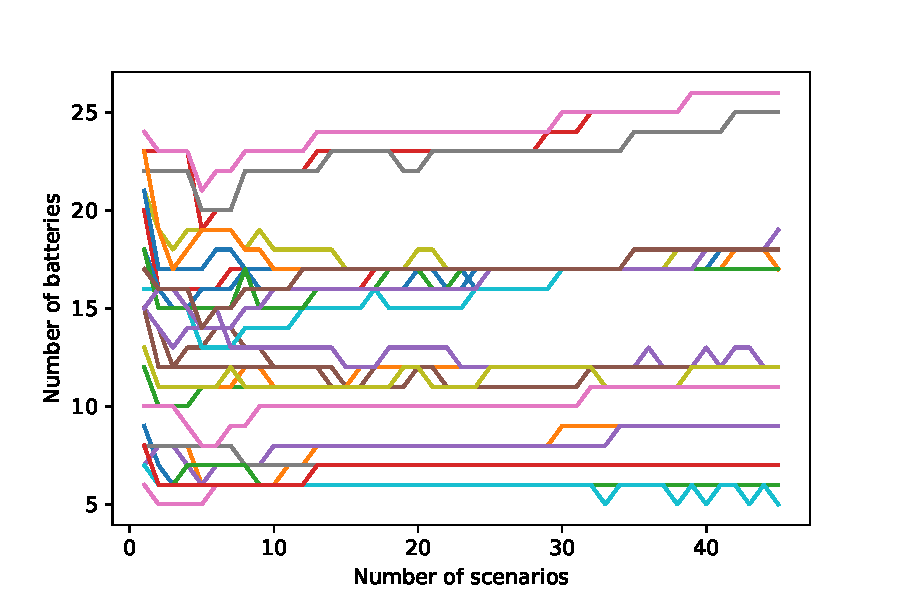
\includegraphics[width=\linewidth]{img/stoc_stac.pdf} 
%   \caption{Changes in the optimal battery size in a community}
%   \label{fig:stoc_change}
% \end{figure}

In Figure \ref{fig:stoc_change}, the change in the optimal battery size for each coalition is plotted as a function of the number of scenarios considered and each line corresponds to one of the different games.
We observe that, in most games, the optimal battery size tends to stabilize around $35-40$ scenarios. This observation shall be employed in future simulations in order to select the number of scenarios. 

We proceed to consider the accuracy of the approximated solution for discrete games.

\subsection{Accuracy of the approximation}

One way to measure the accuracy of the approximation is to consider the empirical value of $\epsilon$ that defines the $\epsilon-core$. If we can compute the value of each of the $2^N - 1$ possible coalitions, then we could check if our approximation is within the core and if so, how far. We will proceed to do so, but only for small values of $N$.

%We can do that by finding the approximated vector in the core and comparing it against the cost of each possible coalition. Clearly, this requires computing the $2^N - 1$ coalitions, which we can only do only for small values of $N$. 
An important observation is that the absolute value of the violation does not satisfactorily capture the accuracy of the approximation: a value of $\epsilon = 1$ when the order of magnitude is a million can be small, but if it is in the order of the tenths it might be too large. To account for this, we consider the value of the violation divided by the total cost of the coalition in which the maximum violation occurs, that is: $\frac{M^{S^*}(y)}{v_d(S^*)}$, where $S^*$ is the coalition for which the maximum violation occurs.

We generated $30$ games for each number of players between $3$ and $10$ (inclusive) using $40$ scenarios in each game.
The box plots in Figure \ref{fig:rel_eps} depict the change in the relative violation of the constraints as the number of players changes. The values are only for the cases when the core of the discrete game is non-empty as it is impossible to measure the distance to the empty set.

As can be seen, as the number of players increases, the violation becomes less meaningful, in line with the results of Lemma ~\ref{lem:bound_error}. This supports the claim that it is better to have larger coalitions, as they are more robust in some sense.

\begin{figure}[]
  \centering


\begin{tikzpicture}
  \begin{axis}
    [
    xtick={1, ..., 8},
    xticklabels={3, ..., 10},
    ytick={0, 0.01, 0.02, 0.03, 0.04},
    boxplot/draw direction=y,
    cycle list name=mycycle,
    height=5cm,
    width=8cm,
    xlabel=Number of players,
    ylabel=$M^{S^*}(y) \slash v_d(S)$,
    ylabel near ticks,
    ]
    
\addplot+[
    boxplot prepared={
      median=0.0,
      upper quartile=0.002768822809964922,
      lower quartile=0.0,
      upper whisker=0.012797056689090027,
      lower whisker=0.0
    }
    ] coordinates {  (1, 0.02697) (1, 0.02859)  };
    
    

    \addplot+[
    boxplot prepared={
      median=0.0018507880769922267,
      upper quartile=0.004958003353515878,
      lower quartile=0.0,
      upper whisker=0.009785297092430048,
      lower whisker=0.0
    }
    ] coordinates {  (2, 0.00999)  };
    
    

    \addplot+[
    boxplot prepared={
      median=0.0,
      upper quartile=0.0015769614275916836,
      lower quartile=0.0,
      upper whisker=0.004944827040169307,
      lower whisker=0.0
    }
    ] coordinates {  (3, 0.00754) (3, 0.00779)  };
    
    

    \addplot+[
    boxplot prepared={
      median=0.0,
      upper quartile=0.000354323883027379,
      lower quartile=0.0,
      upper whisker=0.003621336282185315,
      lower whisker=0.0
    }
    ] coordinates {  (4, 0.00422)  };
    
    

    \addplot+[
    boxplot prepared={
      median=0.0,
      upper quartile=0.0007831394097133494,
      lower quartile=0.0,
      upper whisker=0.002967401506263496,
      lower whisker=0.0
    }
    ] coordinates {  (5, 0.00358)  };
    
    

    \addplot+[
    boxplot prepared={
      median=0.0,
      upper quartile=6.876887603257853e-05,
      lower quartile=0.0,
      upper whisker=0.0005555791048967684,
      lower whisker=0.0
    }
    ] coordinates {  (6, 0.00065)  };
    
    

    \addplot+[
    boxplot prepared={
      median=0.0004191070338928432,
      upper quartile=0.0005886270453638563,
      lower quartile=0.0,
      upper whisker=0.0016845010683056182,
      lower whisker=0.0
    }
    ] coordinates {  (7, 0.00219)  };
    
    

    \addplot+[
    boxplot prepared={
      median=0.0001807248858382736,
      upper quartile=0.00037228681913920996,
      lower quartile=6.703648271528544e-05,
      upper whisker=0.0007441957284442716,
      lower whisker=0.0
    }
    ] coordinates {  (8, 0.00239)  };
  \end{axis}
\end{tikzpicture}

%  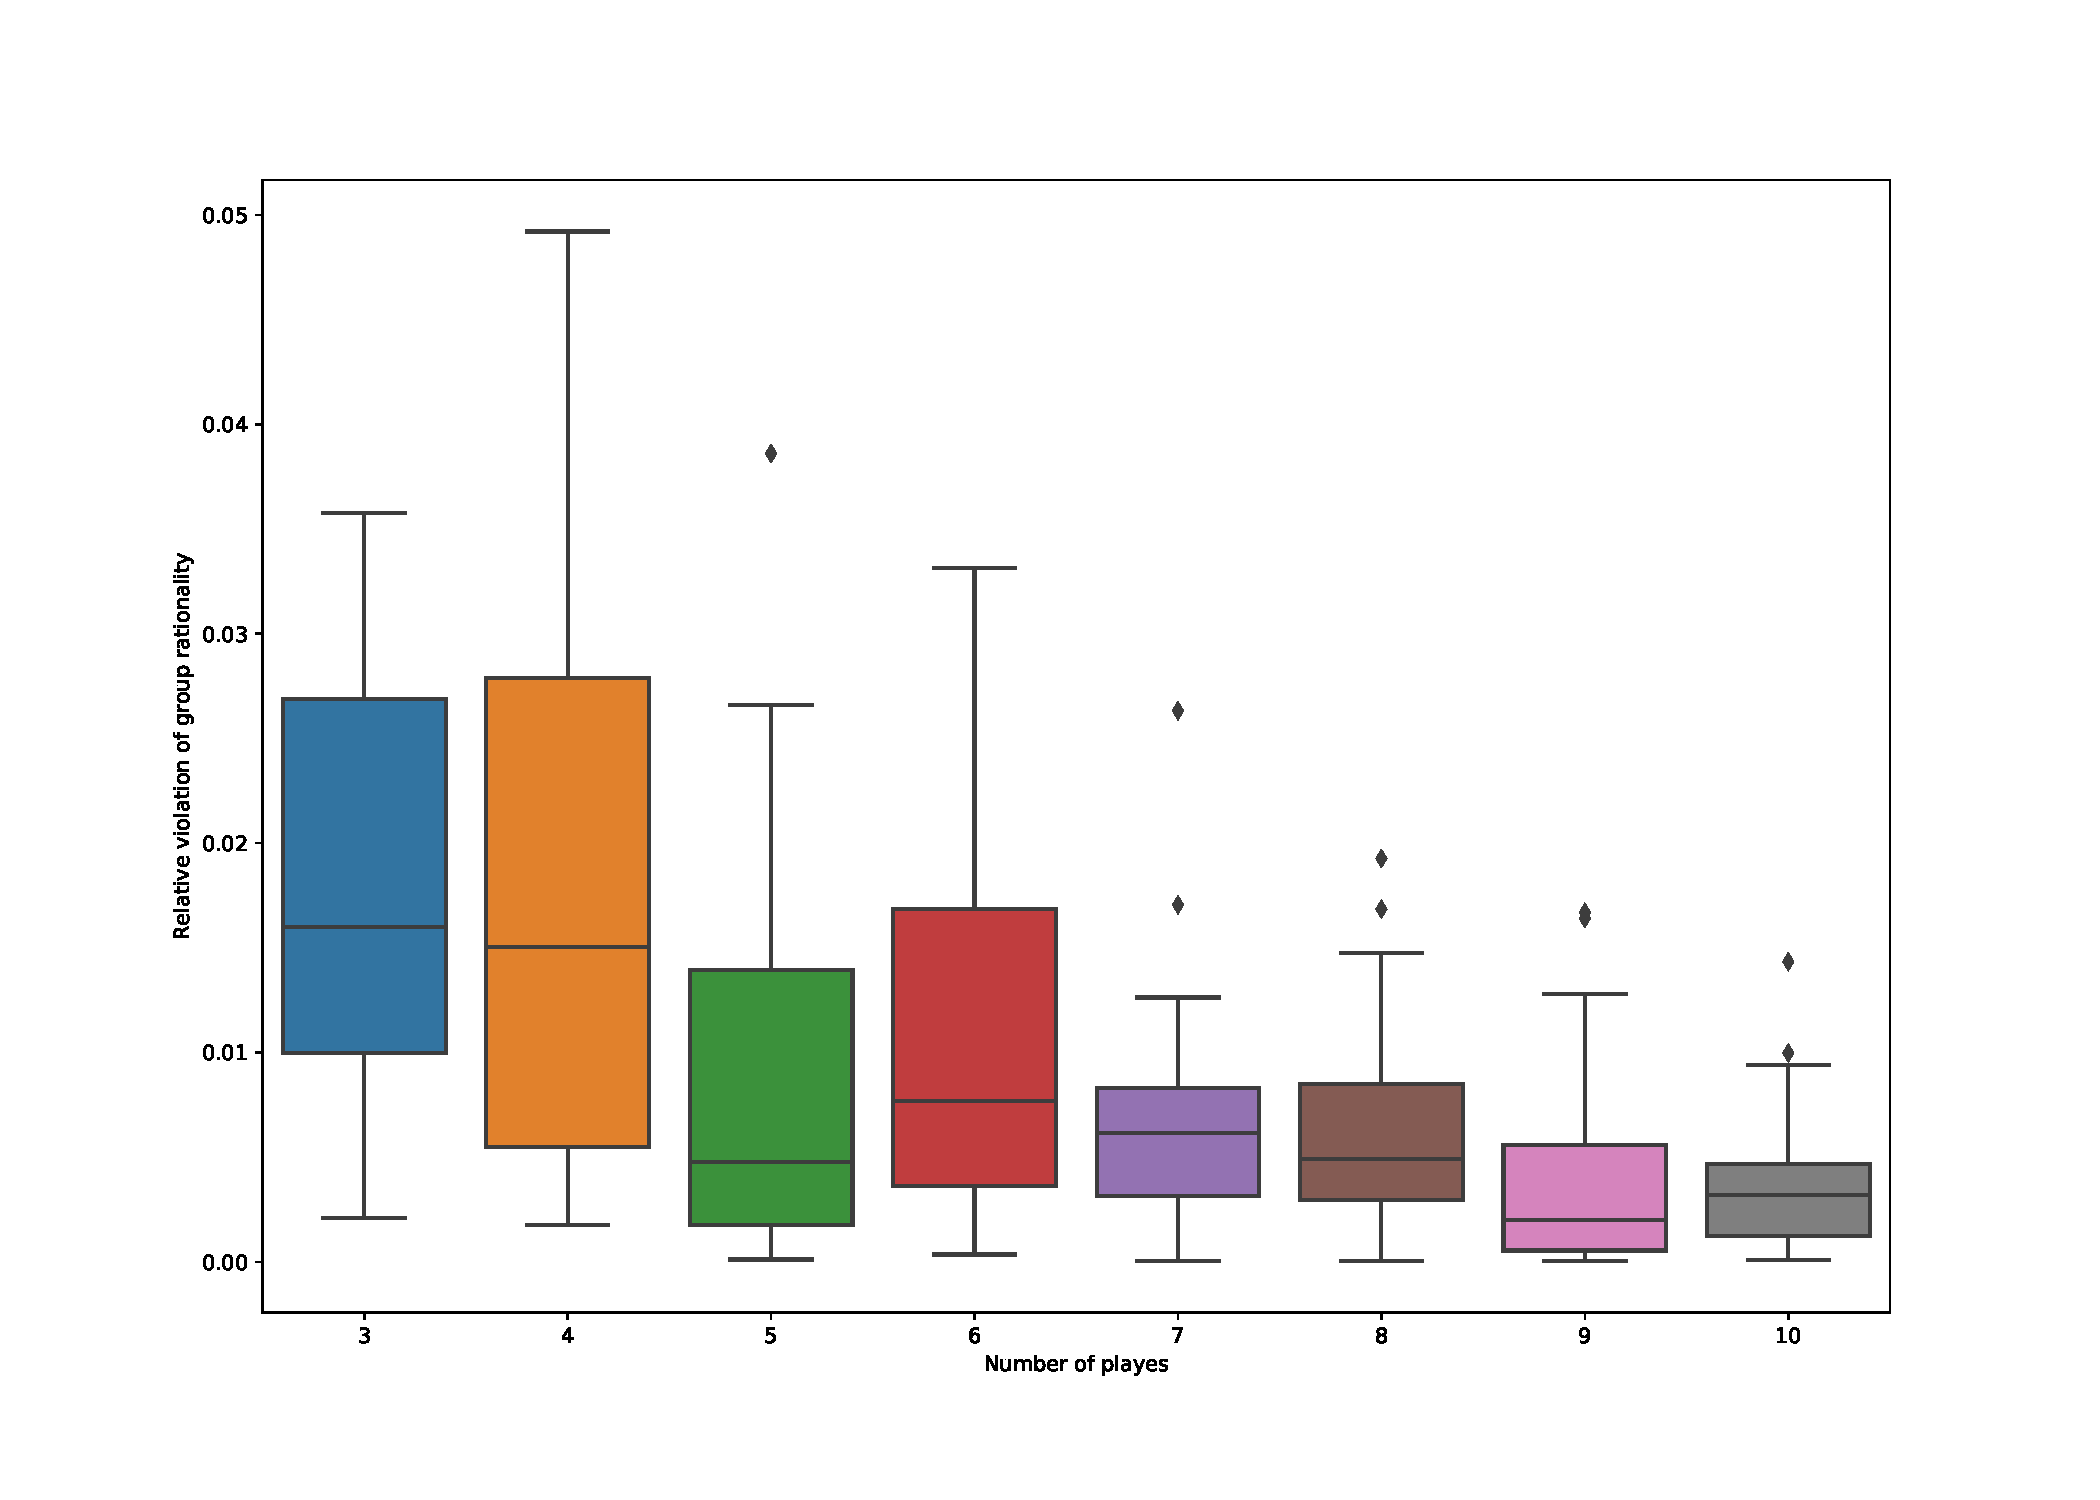
\includegraphics[width=\linewidth]{img/rel_eps.pdf}
  \caption{The relative maximum violation of the approximated solution for a varying number of players}
  \label{fig:rel_eps}
\end{figure}

\begin{table*}[t]
  \centering
  \caption{Comparison of the different cost distribution strategies. In each column the notation $A < B$ indicates the percentage of the players that did worse in $A$ than in $B$. The presented results are the mean and the standard deviation. $N$ stands for the number of consumers, $F$ for the number of test (future) days and $W$ for the number of scenarios.}
  \label{tab:general_performance}
  \resizebox{\linewidth}{!}{\begin{tabular}{lllllllll}
\toprule
   &    &    & $Default$ $<$ $Keep Proportion$ & $Default$ $<$ $Re-solving$ & $Default$ $<$ $Individual$ & $Keep Proportion$ $<$ $Re-solving$ & $Keep Proportion$ $<$ $Individual$ & $Re-solving$ $<$ $Individual$ \\
N & F & W &                                 &                            &                            &                                    &                                    &                               \\
\midrule
15 & 15 & 30 &                 0.59 $\pm$ 0.08 &              1.0 $\pm$ 0.0 &             0.33 $\pm$ 0.2 &                    0.44 $\pm$ 0.06 &                    0.43 $\pm$ 0.08 &                0.33 $\pm$ 0.2 \\
   &    & 45 &                 0.55 $\pm$ 0.15 &              1.0 $\pm$ 0.0 &            0.12 $\pm$ 0.12 &                    0.47 $\pm$ 0.18 &                    0.47 $\pm$ 0.18 &               0.12 $\pm$ 0.12 \\
   & 30 & 30 &                  0.58 $\pm$ 0.1 &              1.0 $\pm$ 0.0 &             0.33 $\pm$ 0.2 &                    0.44 $\pm$ 0.08 &                    0.43 $\pm$ 0.09 &               0.31 $\pm$ 0.19 \\
   &    & 45 &                 0.57 $\pm$ 0.11 &              1.0 $\pm$ 0.0 &            0.12 $\pm$ 0.12 &                    0.43 $\pm$ 0.11 &                    0.45 $\pm$ 0.13 &               0.12 $\pm$ 0.12 \\
30 & 15 & 30 &                 0.55 $\pm$ 0.07 &              1.0 $\pm$ 0.0 &             0.3 $\pm$ 0.17 &                    0.49 $\pm$ 0.05 &                    0.46 $\pm$ 0.06 &                0.3 $\pm$ 0.17 \\
   &    & 45 &                 0.53 $\pm$ 0.08 &              1.0 $\pm$ 0.0 &            0.13 $\pm$ 0.05 &                    0.48 $\pm$ 0.09 &                    0.47 $\pm$ 0.08 &               0.13 $\pm$ 0.05 \\
   & 30 & 30 &                 0.55 $\pm$ 0.05 &              1.0 $\pm$ 0.0 &             0.3 $\pm$ 0.17 &                    0.49 $\pm$ 0.06 &                    0.47 $\pm$ 0.05 &                0.3 $\pm$ 0.17 \\
   &    & 45 &                  \cellcolor{red!25} 0.6 $\pm$ 0.06 &              1.0 $\pm$ 0.0 &            0.13 $\pm$ 0.05 &                    0.45 $\pm$ 0.07 &                    0.42 $\pm$ 0.08 &               0.13 $\pm$ 0.05 \\
45 & 15 & 30 &                 0.55 $\pm$ 0.04 &              1.0 $\pm$ 0.0 &            0.27 $\pm$ 0.15 &                    0.49 $\pm$ 0.05 &                    0.46 $\pm$ 0.04 &               0.27 $\pm$ 0.15 \\
   &    & 45 &                 0.56 $\pm$ 0.06 &              1.0 $\pm$ 0.0 &            \cellcolor{blue!25} 0.12 $\pm$ 0.04 &                    0.46 $\pm$ 0.06 &                    0.44 $\pm$ 0.06 &               0.12 $\pm$ 0.04 \\
   & 30 & 30 &                 0.56 $\pm$ 0.03 &              1.0 $\pm$ 0.0 &            0.27 $\pm$ 0.15 &                    0.48 $\pm$ 0.04 &                    0.46 $\pm$ 0.04 &               0.27 $\pm$ 0.15 \\
   &    & 45 &                  0.6 $\pm$ 0.03 &              1.0 $\pm$ 0.0 &            0.12 $\pm$ 0.04 &                    0.43 $\pm$ 0.04 &                    0.41 $\pm$ 0.03 &               0.12 $\pm$ 0.04 \\
\bottomrule
\end{tabular}
}
\end{table*}

\subsection{Overall performance}\label{sub:gp}

We conclude the numerical evaluation by considering the overall performance of the model. A central question is whether the cooperative game can be an efficient method for increasing the number of storage devices in the power grid without outside incentives.

To do so, two measures are needed, namely: the economic benefit of each consumer of participating in the coalition, and the number of extra storage units that are installed.

%of out-of-sample days used to evaluate the %performance changes.
We simulated 96 coalitional storage games, varying the number of players $N \in \{15, 30, 45\}$, the number of scenarios used for making the decision $|\Omega| = W \in \{30, 45\}$ and the number of days after the investment in which the decision was evaluated $F \in \{15, 30\}$. For each combination of parameters, 8 games were created by sampling the load profile of different users.

For the two techniques used to distribute the costs during the test days and the two benchmarks, Figure \ref{fig:performance1} depicts the total cost of 10 of the players for one such game. Although some of the players do much better by joining the coalition, others are worse off.
In particular, observe that for player 4 the technique is very negative, while for player 6 it is highly profitable. This can happen if the scenarios do not adequately represent the loads of each user and the investment is made with consumption profiles that are not very representative of the average consumption of those users. One example of that is assigning the same probability to an extreme peak of consumption.  For example, if the average consumption of a player is X kWh per day but the scenarios used to determine the cost division coincide with all the days in which he/she consumes above $X$, then the outcome will not be favourable for he/she.
\begin{figure}[h]
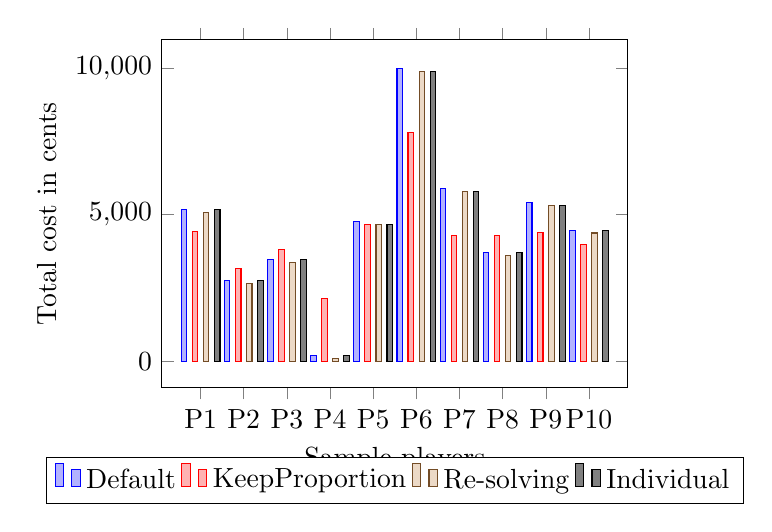
\begin{tikzpicture}
\begin{axis}[
x tick label style={
/pgf/number format/1000 sep=},
xtick={0, ..., 9},
xticklabels={P1, P2, P3, P4, P5, P6, P7, P8, P9, P10},
yticklabel style={
        /pgf/number format/fixed,
        /pgf/number format/precision=5
},
scaled y ticks=false,
%ytick={0, 1000, ..., 10000},
%yticklabels={0, 1000, ..., 10000},
ylabel=Total cost in cents,
xlabel=Sample players,
%enlargelimits=0.15,
legend style={at={(0.5,-0.20)},
anchor=north,legend columns=-1},
ybar,
bar width=2pt,
ylabel near ticks,
width=7.5cm,
height=6cm,
]
\addplot coordinates {
(0, 5164.085) (1, 2741.558) (2, 3459.796) (3, 177.717) (4, 4765.9) (5, 9975.363) (6, 5895.572) (7, 3702.434) (8, 5415.379) (9, 4463.329)
};


\addplot coordinates {
(0, 4417.117) (1, 3149.594) (2, 3821.339) (3, 2124.824) (4, 4656.924) (5, 7792.349) (6, 4279.182) (7, 4272.654) (8, 4377.481) (9, 3989.703)
};


\addplot coordinates {
(0, 5070.485) (1, 2647.958) (2, 3366.196) (3, 84.117) (4, 4672.3) (5, 9881.763) (6, 5801.972) (7, 3608.834) (8, 5321.779) (9, 4369.73)
};


\addplot coordinates {
(0, 5164.085) (1, 2741.558) (2, 3459.796) (3, 177.717) (4, 4657.9) (5, 9867.363) (6, 5787.571) (7, 3702.434) (8, 5307.379) (9, 4463.329)
};
\legend{Default, KeepProportion,Re-solving, Individual}
\end{axis}
\end{tikzpicture}


% \begin{figure}[h]
%   \centering
%  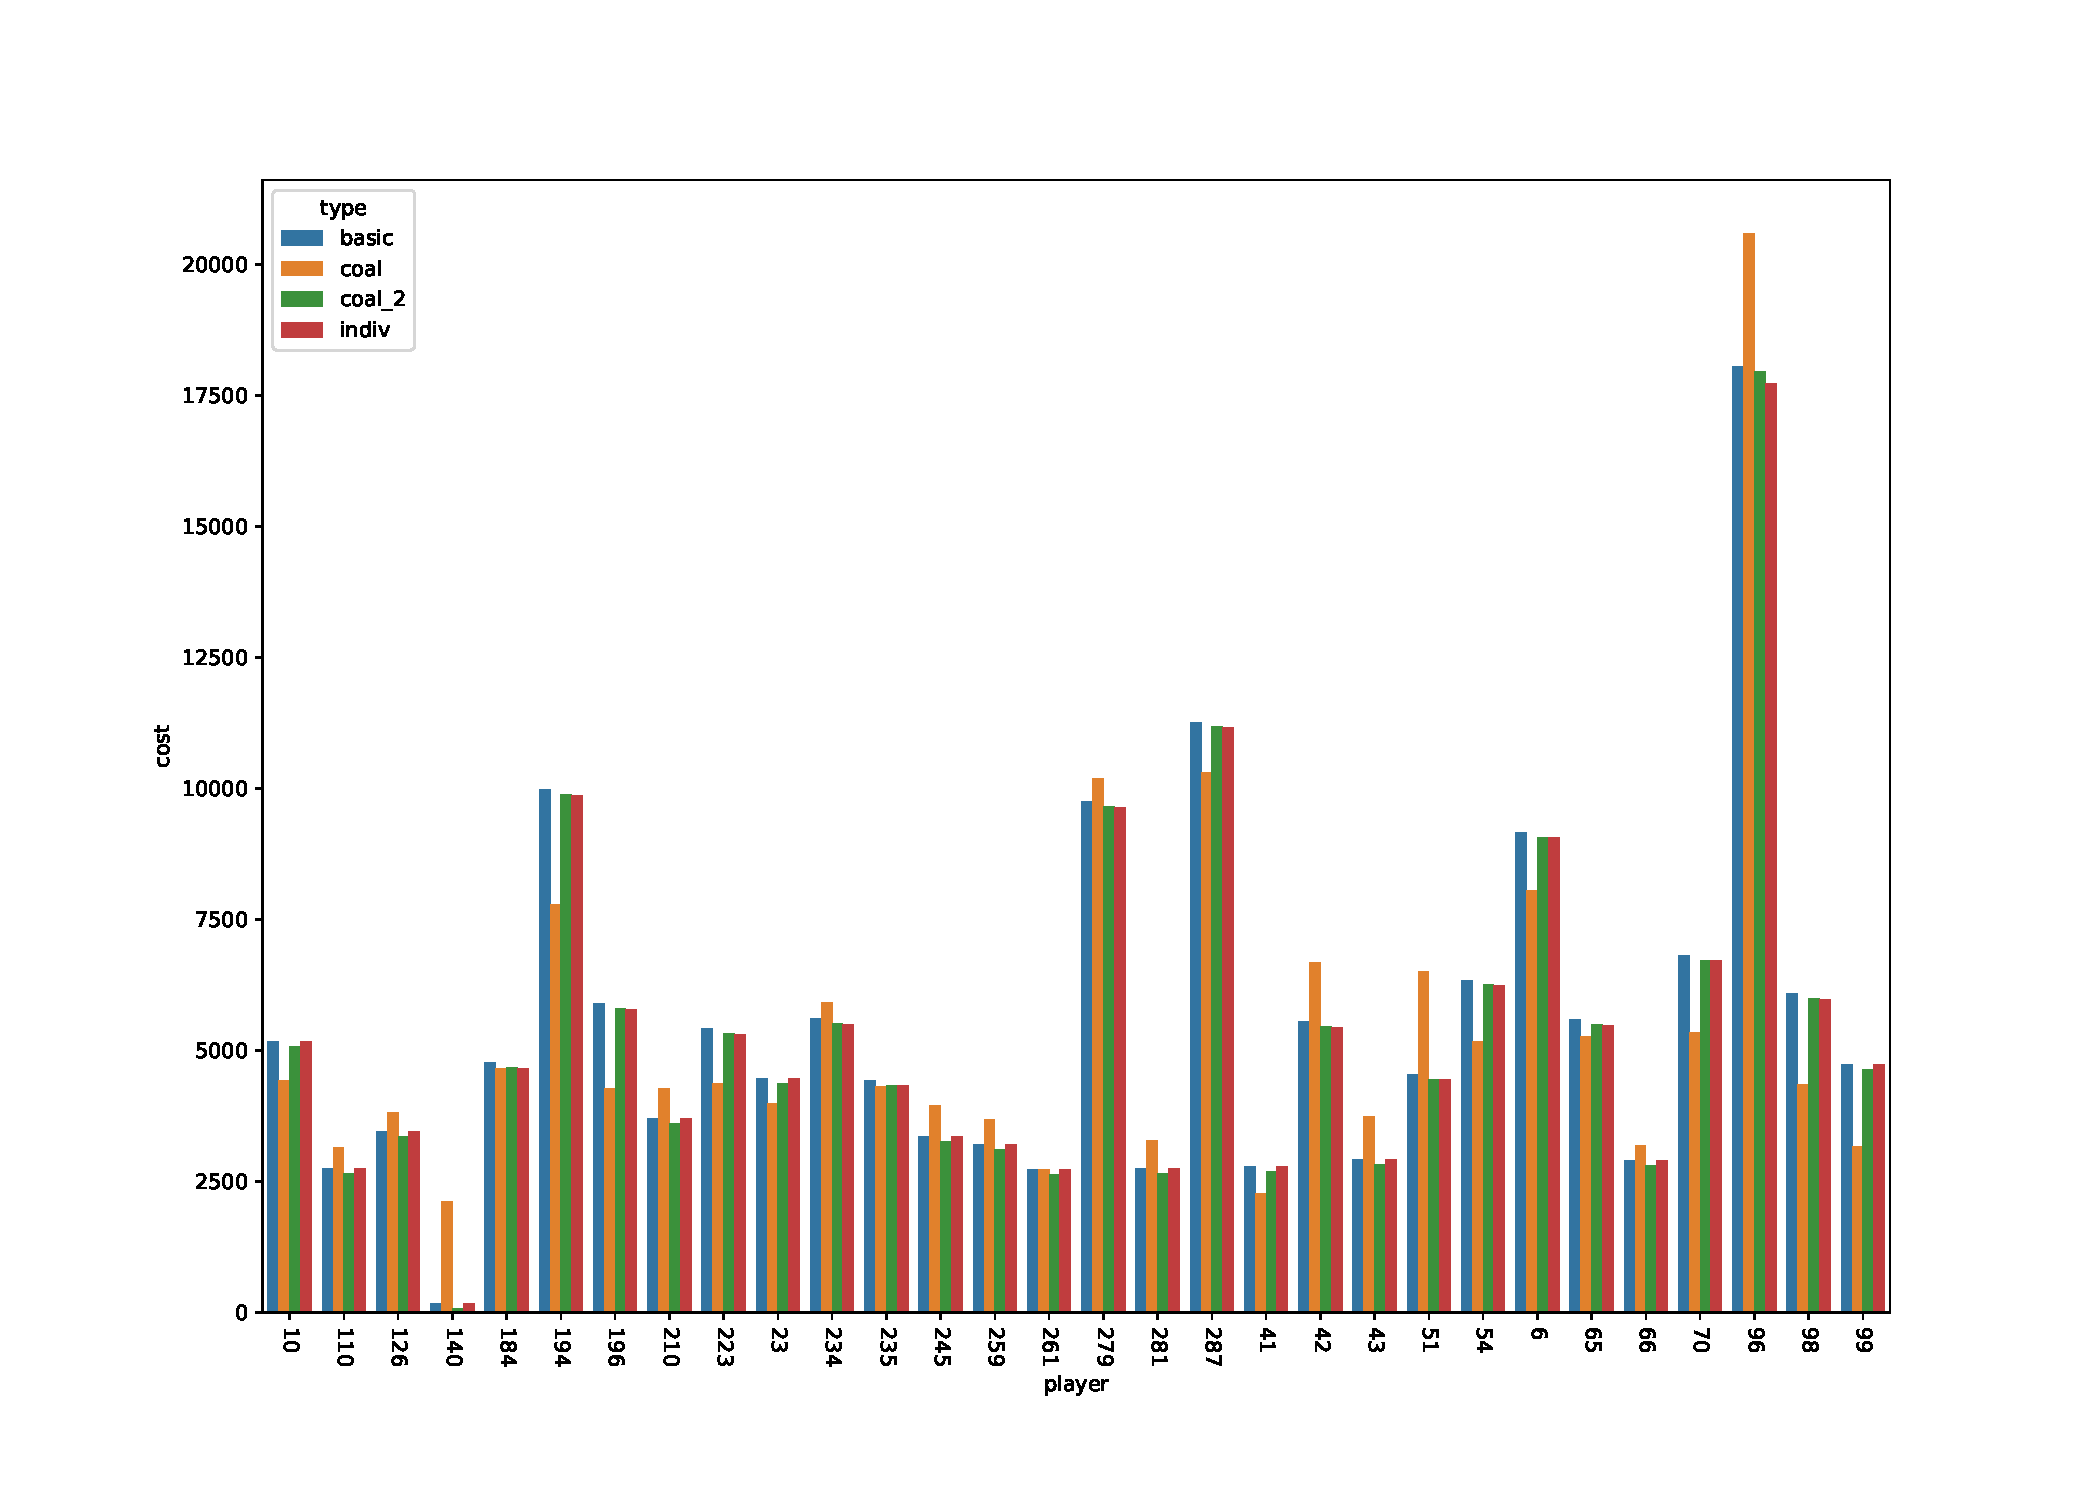
\includegraphics[width=\linewidth]{img/gp_1.pdf} 
  \caption{The total cost of individual players for 15 days after the investment using the different techniques to assign the cost.}
  \label{fig:performance1}
\end{figure}

A thorough assessment of the performance is provided in Table ~\ref{tab:general_performance}. For each combination of the considered parameters, the table depicts the percentage of users (on average) that are better off by using one cost assignment technique over the other.
As an example, consider the two highlighted cells in the table. The blue one indicates that, for the simulations with $45$ consumers, $45$ scenarios and $15$ test days, only $12\%$ of the consumers preferred the \textbf{Individual} investment over the \textbf{Default} one (all the rest preferred the \textbf{Default}). On the other hand, the red cell indicates that $60\%$ of the players preferred the \textbf{Keep Proportion} technique versus doing nothing, in the games with $30$ players, 30 test days and 45 scenario days.
We observe that the \textbf{Keep Proportion} technique has very different outcomes: for about half of the players it is profitable, yet for the other half it is not.  Nevertheless, we observe that not investing at all in storage is \emph{always} worse than joining the grand coalition and paying a cost calculated using the \textbf{Re-solving} technique.



Furthermore, we consider the increase in storage owned by the players while participating in the cooperative scheme. For the same scenarios as in Table \ref{tab:general_performance}, Table \ref{tab:cant_bats} depicts the average increase in the number of batteries and the percentage of change. It can be seen that cooperation duplicates or even triplicates the number of storage owned by players in consideration (with respect to buying storage individually). Furthermore, knowing that using the payment scheme \textbf{Re-solving} no player is worse than doing nothing, we conclude that coalitional storage games are capable of increasing the amount of storage in the community while satisfying individual needs.

\begin{table}
  \begin{tabular}{lllrr}
\toprule
   &    &    &  Averge difference &  Percentage of increase \\
N & F & W &                    &                         \\
\midrule
15 & 15 & 30 &                3.8 &                     inf \\
   &    & 45 &                4.4 &                     inf \\
   & 30 & 30 &                3.8 &                     inf \\
   &    & 45 &                4.4 &                     inf \\
30 & 15 & 30 &                8.1 &                  232.63 \\
   &    & 45 &                8.4 &                  374.67 \\
   & 30 & 30 &                8.1 &                  232.63 \\
   &    & 45 &                8.4 &                  374.67 \\
45 & 15 & 30 &               12.8 &                  242.51 \\
   &    & 45 &               12.4 &                  373.10 \\
   & 30 & 30 &               12.8 &                  242.51 \\
   &    & 45 &               12.4 &                  373.10 \\
\bottomrule
\end{tabular}

  \caption{Changes in the number of batteries between individual and cooperative investments.}
  \label{tab:cant_bats}
\end{table}


\section{Conclusions and Future Work}

In this study we extended the coalitional storage game for modeling the shared investment in storage. We provided two extensions, namely, considering discrete battery sizes and accommodating a stochastic representation of the load. We believe that these extensions are important steps towards the deployment of the theoretical findings of this line of work in real-life settings.
We have shown that the cooperative investment is always profitable when continuous batteries are considered and almost always profitable in the case of discrete batteries.
Furthermore, we provided computationally-efficient algorithms for finding such solutions. These solutions specify how the costs should be split among players.

It follows from our theoretical model that the shared investment is profitable for players when their real consumption distribution is taken into account. Unfortunately, our numerical results indicate that using an approximation of such consumption profiles can lead to unsatisfied players in the long run. Thus, constructing better approximations of the considered profiles is one of our intended directions for future work.
% Our numerical simulations indicate that the stochastic consumption scenario selection plays a key role in the performance of the model. Indeed, we observed that simply using the Cartesian product of past consumption profiles as the set of scenarios can lead to unsatisfied users in the long run. This can be surmounted by appropriately designing the scenarios in a representative way, which is a subject for future research.

In our numerical simulations, the cooperative scheme achieved an increase between $100\%$ and $250\%$ in the amount of storage hosted in residential premises compared to the setting in which consumers invest individually, when it was profitable for them to do so. Accordingly, we believe that coalitional games offer solution concepts that are very well positioned to boost the number of distributed storage devices in Smart Grids. Furthermore, some consumers might consider the tasks of installing storage in their homes overly complicated. In such a case, opting to participate in collective storage (which might not require more than a simple agreement) may offer a more attractive approach to adopting storage.

It is important to note that a coalitional game cannot make a battery profitable if the gap between the high price and the low price of electricity is lower than the amortized cost of the battery. That is, the viability of buying storage first depends on the electricity tariffs and on the storage prices, and obviously our model (and its implied scheme) cannot get around this problem. Nevertheless, if storage is barely profitable, participating in a shared investment will provide higher margins of profit at a reduced risk (which is shared among the members of the coalition).
Relatedly, we expect battery technologies to improve and decrease their costs in the future, hence increasing the applicability of the cooperative game approach proposed in this study.

Our study indicates several directions for future research that could further increase the benefits of the proposed solution.  One such is to consider advance tariff models, for example those that include peak demand charges; another is to find efficient schemes to update an existing coalition once either new players wish to join or present ones wish to leave. Finally we are considering the substitution of the second-stage optimization problem in our model with a more detailed version, such as the one used in \cite{hashmi2019}, \cite{kiedanskiforecast}.

\bibliographystyle{ACM-Reference-Format}
\bibliography{acmart}

%\pagebreak
\appendix

%\textbf{APPENDICES}

\section{Matrix formulation of the optimization problem}\label{ap:matrix}

In this appendix we provide the matrices and vectors involved in the matrix formulation of the linear optimization problem \eqref{eq:cost_lp}.
%\subsection{Continuous and deterministic}

\begin{equation}
  \acd = \begin{bmatrix} 
    \delta & 0 & 0 & 1 & - 1 & 0 & 0 & \dots & 0 \\
    \delta & 0 & 0 & 0 & 0 & 1 & -1 & \dots & 0 \\
    \vdots & \vdots & &&&&& \vdots\\
    (1 - T\ramp) & 1 & -1 & 0 & 1 & 0 & 1 & \dots  \\ 
    \end{bmatrix}
\end{equation}

such that $\acd \in \mathbb{M}_{(T+1)\times (2T + 3)}$

\begin{equation}
    \bcd = \begin{bmatrix}
    x^S_1 \\
    x^S_2 \\
    \vdots \\
    x^S_{T} \\
    0
    \end{bmatrix}
    \qquad 
    \text{ with }\sum_{n \in S} \cons^n_t = \cons^S_t
\end{equation}


\begin{equation}
    \mathbb{R}^{2T + 3} \ni \ccd = \begin{bmatrix}
    -(\pi + \pricelow) & -\pricehigh & \pricelow &  -\pricehigh & 0 & -\pricehigh & \dots & 0\\ 
    \end{bmatrix}
\end{equation}


\section{Proof of Proposition \ref{prop:equiv}}\label{ap:equiv}

\begin{paragraph}{Proposition \ref{prop:equiv}}
The optimization problems \eqref{eq:cost_coal} and \eqref{eq:cost_lp} are equivalent.
\end{paragraph}


\begin{proof}
The basic idea is as follows: each variable $\ep_t, \ene_t$ allows us to represent the minimum inside the summation in Equation \eqref{eq:cost_coal_bat}, while $\Ep, \Ene$ represent the outer minimum.

Specifically, by Equation \eqref{cons:ramp}: $\min\{ \delta B, x^S_t \} = \min\{ \delta B, \delta B + \ep_t - \ene_t \} = \min\{ \delta B, \delta B - \ene_t \} = \delta B - \ene_t$. \\
Doing some extra arithmetic we obtain that:

\begin{equation*}
\begin{aligned}
&\min\left\{ B, \sum_{t=\frac{\mathcal{T}}{2}}^{\mathcal{{T}}} \min\{x^S_t, \delta B\} \right\} = \min\{ B, \sum_t \delta  B - \ene_t \}\\
&= \min\{ B, B + \Ep - \Ene\} = B - \Ene
\end{aligned}
\end{equation*}

\begin{equation}
    \begin{aligned}
      v^S(\Bat) &= \frac{BP}{L}   + p^ h\sum_{t=\frac{\mathcal{T}}{2}}^{\mathcal{{T}}} x^S_t 
  - (p^h -p^l)(B - \Ene)   \\
  &= \frac{BP}{L} + \pricelow (B - \Ene)   + p^ h\sum_{t \in \mathcal{T}} x^S_t - \pricehigh(B - \Ene) \\
  & = \frac{BP}{L} + \pricelow (B - \Ene) + \pricehigh \sum_t (\delta B + \ep_t - \ene_t) \\
  &- \pricehigh((\sum_t (\delta B - \ene_t) - \Ene) \\
  & =  \frac{BP}{L} + \pricelow (B - \Ene) + \pricehigh (\Ep + \sum_t \ep)
    \end{aligned}
\end{equation}

\end{proof}

\section{Stochastic LP formulation}\label{ap:largestoc}

In this appendix we formulate the large linear optimization problem \eqref{opt:large_lp} that is obtained by merging the optimization problem associated with the first stage \eqref{eq:stoc_first_stage} and second stage \eqref{opt:second_stage} of the stochastic formulation of the cost of a coalition. 

\begin{mini}[3]
{\bat, \Ep, \Ene, \ep, \ene}{\costbat \bat + \sum_{w \in \Omega} p(w) C(\bat, \Ep, \Ene, \ep, \ene, w)}{}{P_S)}\label{opt:large_lp}
\addConstraint{\ramp\bat + \ep_t(w) - \ene_t(w)}{ = \sum_{n \in S} \cons^n_t(w)}{ \ \forall t \in \mathcal{T}, \ \forall w \in \Omega}
\addConstraint{\bat + \Ep(w) - \Ene(w)}{= \sum_t (\ramp\bat - \ene_t(w))}{, \ \forall w \in \Omega}
\addConstraint{\bat, \Ep, \Ene, \ep, \ene}{\geq 0}{}
\end{mini}

where:

\[
C(\bat, \Ep, \Ene, \ep, \ene, w) = \pricelow(\bat - \Ene(w)) +  \pricehigh(\Ep(w) + \sum_t \ep_t(w))
\]

\section{Proof of Theorem \ref{th:batterysize_round}}\label{app:batterysize}


\begin{paragraph}{Theorem \ref{th:batterysize_round}}
The optimal battery size for a coalition $S$ in the discrete setting is given by $B^{\uparrow}$ or $B^{\downarrow}$, where $B^{\uparrow}$ is the smallest multiple of $B$ greater than $\beta$ and $B^{\downarrow}$ is the largest positive multiple of $B$ smaller or equal than $\beta$. In this context, $\beta$ is the optimal battery size for the coalition in the continuous setting.
\end{paragraph}
\begin{proof}
Consider a parametric linear program $\min\{ cx | Ax = b + \hat{b}\lambda, x\geq 0\}$. It is known that if $\phi(\lambda)$ is the value of the optimal solution, then $\lambda \to \phi(\lambda)$ is a convex piecewise linear continuous function \cite{Adler1992}.
Observe that the optimization problem considered so far can be written in this parametric form, where the parameter $\lambda$ is precisely the battery size $\bat$ (the reformulation requires to replace all the instances of $\bat$ in the cost function by the appropriate combination of the rest of the variables).

Since $\phi$ is continuous and convex in $R^+$ and, furthermore
$\lim_{x\to\infty} \phi(x) = \infty$, $\phi$ has a global minimum that coincides with the battery size in the continuous case. Now, because $\phi$ is convex, it holds that, among the integer values, $\phi$ has to be minimized by either $\bat^{\uparrow}$ or $\bat^{\downarrow}$. This implies that, instead of solving the mixed integer optimization problem, it suffices to solve the continuous one and check which of the two solutions is better.
\end{proof}

\section{Proof of Stochastic Balance}\label{app:stoc_balanced}

This appendix provides the proof of Theorem \ref{th:stoc_balanced}.

\begin{paragraph}{Theorem \ref{th:stoc_balanced}}
The cooperative game defined by using optimization problem \eqref{opt:large_lp} as the cost of each coalition is balanced and, therefore, it has a non-empty core. 
\end{paragraph}

\begin{proof}
For the continuous and stochastic version of the problem we shall use the notation $\acs, \bcs, \ccs$ to denote the components of the matrix formulation of the associated LP.
Furthermore, let $W = |\Omega|$.

The proof is quite similar to that of the deterministic case. Observe that the main difference between the feasible sets of optimization problems \eqref{opt:large_lp} and \eqref{eq:cost_lp} is that in the former, each constraint is repeated for each scenario $w \in \Omega$. Therefore, we shall show that the same ideas used in the proof of Theorem \ref{th:core-cd} still hold when each constraint is also indexed by $w$. First,  we show that the consumption profiles are still additive while multiplying them by the \textit{balanced coefficients} (Equation \eqref{eq:stoc_proof_1}):

\begin{equation}\label{eq:stoc_proof_1}
\begin{aligned}
      &\sum_S \alpha(S) x^S_t(w)  = \sum_S \alpha(S) \sum_{n \in S}x^n_t(w) \\ &= \sum_{n \in N}x^n_t(w)\sum_{S \colon i \in S} \alpha(S) = \sum_{n \in N} x^n_t(w) = x^N_t(w)
\end{aligned}
\end{equation}

Finally, we show that the \textit{balanced} solution is still feasible for the Grand Coalition problem \eqref{eq:stoc_proof_2}.

\begin{equation}\label{eq:stoc_proof_2}
\begin{aligned}
    &\acs \left(\sum_S \alpha(S) y_S \right) = \sum_S \alpha(S) \left( Ay_S \right) = \\ &= \sum_S \alpha(S) \begin{bmatrix} x^S_1(w_0) \\ \\ \vdots \\ x^S_T(w_0) \\ 0 \\ x^S_1(w_1)\\ \vdots \\ x^S_T(w_W) \\ 0 \end{bmatrix} = \begin{bmatrix} \sum_S \alpha(S) x^S_1(w_0) \\ \\ \vdots \\  \sum_S \alpha(S) x^S_T(w_0) \\ \sum_S \alpha(S) 0 \\ \sum_S \alpha(S) x^S_1(w_1)\\ \vdots \\ \sum_S \alpha(S) x^S_T(w_W) \\ \sum_S \alpha(S) 0 \end{bmatrix} = \begin{bmatrix} x^N_1(w_0) \\ \\ \vdots \\ x^N_T(w_0) \\ 0 \\ x^N_1(w_1)\\ \vdots \\ x^N_T(w_W) \\ 0 \end{bmatrix}
\end{aligned}
\end{equation} 
\end{proof}



\end{document}
\endinput
%%
%% End of file `sample-sigconf.tex'.
